\documentclass{unicam_thesis}

\usepackage[utf8]{inputenc}
\usepackage{listings}
\usepackage[inkscapeformat=png]{svg}
\usepackage[backend=bibtex]{biblatex}

% config
\nocite{*}
\bibliography{biblio.bib} %or \addbibresource{biblio.bib}
\graphicspath{{Immagini}}
\lstset{
    % basicstyle=\ttfamily,
    % postbreak=\raisebox{0ex}[0ex][0ex]{\BeginAccSupp{ActualText={}}\ensuremath{\color{gray}\hookrightarrow\space}\EndAccSupp{}},
    columns=fullflexible,
    breaklines=true
}

%%%%%%%%%%%%%%%%%%%%%%%%%%%%
% TESI DATI FRONTESPIZIO
%%%%%%%%%%%%%%%%%%%%%%%%%%%%

\title{Servizi Onion \\ Dalla teoria all'implementazione }

\university{Universit\`a degli Studi di Camerino}%
\school{Scienze e Tecnologie}%
\course{Laurea in Informatica (Classe L-31)}%

\author{Leonardo Migliorelli}%
\advisor{Fausto Marcantoni}%
\coadvisor2{Correlatore Name}%
\academicyear{2022/2023}%
\matricola{113920}%

%%%%%%%%%%%%%%%%%%%%%%%%%%%%
% FINE DATI FRONTESPIZIO
%%%%%%%%%%%%%%%%%%%%%%%%%%%%

\makeindex
\theoremstyle{definition} \newtheorem{esempio}{Esempio}[chapter]
\theoremstyle{definition} \newtheorem{definizione}{Definizione}[chapter]
\theoremstyle{plain} \newtheorem{teorema}{Teorema}[chapter]


\begin{document}
\maketitle

\tableofcontents
\lstlistoflistings
\listoffigures
\listoftables

\makeatletter \def\input@path{{Capitoli/}}
    \chapter{Introduzione}
\label{chap:intro}

Le moderne tecnologie di rete consentono una rapida comunicazione da ogni parte del mondo, avvicinando culture altrimenti distanti migliaia di chilometri. Due dei più grandi temi del nostro secolo sono la privacy e l'anonimato, in particolare parlando di reti internet ogni connessione tra client e server passa per una moltitudine di router che conoscono esattamente l'indirizzo (e quindi l'identità) del mittente e del destinatario. Con un pò di conoscenze non è complicato scoprire questi dati e sfruttarli a proprio vantaggio, le stesse big company spesso usano l'indirizzo IP con cui ci si connette al loro sito per tracciare l'utente e fornirgli articoli e pubblicità mirata o vendere i medesimi dati a terzi. 
La Rete Onion è stata creata per risolvere esattamente questo problema, implementando le giuste tecnologie per proteggere gli utenti dall'analisi del traffico e dalle intercettazioni


\section{Motivazione}
\section{Obiettivi}

La tesi ha come principale obiettivo la specifica della rete onion, dalle mix networks alla prima versione di Onion fino a Onion v3 e la relativa implementazione di un servizio completo

\section{Struttura della Tesi}


    \chapter{Onion Routing}
\label{chap:Capitolo1}

\begin{figure}[htpb!]
    \centering
    \includesvg[width=\textwidth]{SpiegazioneOnion.svg}
    \caption{Vita di un pacchetto onion}
    \label{fig:routing}
\end{figure}

La \textbf{rete onion} è una rete distribuita composta dall'insieme di \textbf{router onion} che agiscono come nodi di rete e collaborano per portare un pacchetto dalla sorgente alla destinazione. Il tutto avviene senza che nessun nodo possa conoscere contemporaneamente l'host sorgente e l'host di destinazione, grazie alla criptografia a strati del pacchetto, per cui ogni strato viene criptato con una chiave differente e può essere decriptato solo dal nodo con la stessa chiave simmetrica, scoprendo cosi le informazioni sul prossimo nodo. Il nodo finale (exit node) può infine decriptare l'intero messaggio e scoprirne il corpo. Questo meccanismo è derivato dallo studio di David Chaum riguardo alle mix networks. La risposta del pacchetto segue lo stesso criterio sfruttando nodi, algoritmi e chiavi differenti. Questo concede all'utilizzatore di rimanere completamente anonimo, cosa che non può essere avvenire con la semplice criptografia SSL che agisce esclusivamente sul corpo del messaggio \\
Come prima operazione per utilizzare la rete onion il client deve generare un nuovo circuito definendo il percorso di nodi che ogni pacchetto dovrà seguire, iniziando dal primo nodo vengono scambiate informazioni crittografiche come l'algoritmo e le chiavi da usare, poi si usano le informazioni finora ottenute per ottenere quelle del prossimo nodo e cosi via fino a che non si è generato tutto il circuito, grazie a questo meccanismo neanche durante la generazione del circuito è possibile risalire al client. Viene usata la crittografia asimmetrica per scambiare le chiavi simmetriche tra il client e ogni router, questo viene fatto in quanto la crittografia asimmetrica è molto costosa e viene quindi usata solo alla generazione del circuito, successivamente gli strati vengono criptati e decriptati con la stessa chiave simmetrica. Questo consente alla rete onion ad avere una bassa latenza che è incrementata solo dal numero di onion router nel percorso e non dalla tecnologia che non è distante da quella usata in HTTPS 
\cite{OnionRouting}

\newpage
\section{Applicazioni di utilizzo}
L'onion routing può essere usato con una moltitudine di protocolli e applicazioni, tra i più comuni troviamo HTTP(S), FTP, SSH, SMTP, DNS e VPNs. L'utilizzo di molti dei protocolli più comuni avviene tramite gli onion proxies, i quali sono suddivisi in tre proxy layer logici
\begin{itemize}
    \item Un proxy che genera e gestisce le connessioni, per operare ha necessità di conoscere la topologia e i percorsi verso altri nodi, tutte le informazioni vengono distribuite in modo sicuro all'interno della rete a ogni nuovo nodo che si connette 
    \item Un proxy chiamato \emph{\textbf{“Application Specific Proxy”}}, a una connessione la relativa applicazione invia al proxy il pacchetto che normalmente invierebbe al server di destinazione, il proxy si occupa di convertire lo stream di dati in un formato accettato dalla rete onion
    \item Un proxy opzionale chiamato \emph{\textbf{“Application Specific Privacy Filter”}} che sanifica lo stream di dati rimuovendo informazioni che potrebbero identificare la sorgente
\end{itemize}

\cite{OnionRouting} \\
I proxy possono essere configurati in molteplici modi, tra i quali vi è la possibilità di eseguire il proxy in un server remoto e sfruttare la rete Tor senza dover installare il software in ogni dispositivo, che quindi non ne deve gestire la computazione

\newpage
\section{Onion come Mix Network}
La rete Tor è una delle molteplici reti basate sullo studio di David Chaum sulle Mix network, il suo studio si concentrò sulla rete basata sulla crittografia asimmetrica e sui sistemi di risposta senza conoscere l'identità del destinatario. Tutta la rete doveva funzionare senza necessità di un'ente centrale a gestire le connessioni. \\
In particolare abbiamo chiave pubblica K e chiave privata P, abbiamo inoltre
\begin{itemize}
    \item K(x) la funzione che cripta x con la chiave pubblica, può solo essere decriptato con la chiave P
    \item P(x) la funzione che cripta x con la chiave privata, può solo essere decriptato con la chiave K
\end{itemize}
Abbiamo quindi $P(K(x)) = K(P(x)) = x$ \\
Con questa tecnica però qualcuno potrebbe determinare il contenuto di un messaggio creando una copia identica in quanto $y = x → K(y) = K(x)$, per risolvere questo problema si esegue la crittografia del messaggio inserendo una stringa casuale R ottenendo quindi chiavi sempre diverse tramite le funzioni $K(x,R)$ e $P(x,R)$, questa tecnica è chiamata sealing \\
In una rete questo sistema viene implementato in maniera ridondante, il messaggio M viene criptato insieme a una stringa casuale R con la chiave pubblica del destinatario Kb, il tutto viene criptato assieme all'indirizzo B e a una stringa casuale R1 con la chiave pubblica K1 del nodo 1, questo processo potrebbe essere esteso con N nodi (mix) rendendo quindi la rete molto sicura \ 
$K1(R1, Kb(R0, M), B)$ \\
Quando il nodo 1 riceve il pacchetto lo decripta con la sua chiave privata scartando R1 ottiene $Ka(R0, M), B$. Inoltra quindi il nuovo pacchetto a B \\
Il destinatario di un pacchetto deve avere la possibilità di rispondere senza conoscere l'indirizzo di A. \\
A sfrutta il proprio indirizzo reale per generare un indirizzo non tracciabile, in particolare genera due chiavi pubbliche Ka e R1, cripta il proprio indirizzo A assieme alla chiave R1 come stringa casuale usando la chiave del mix \\
$K1(R1, A), Ka$ \\
Quando B deve rispondere al pacchetto usa Ka per criptare il messaggio e $K1(R1, A)$ come indirizzo di destinazione, il mix M1 che riceve il pacchetto usa la chiave privata P1 per decriptare l'indirizzo di destinazione (A) ed usa la stringa casuale R1 come ulteriore chiave per criptare il messaggio \\
$K1( R1, A ), Ka( R0, M ) => A, R1( Ka( R0, M ) )$ \\
Con questo sistema B può rispondere ad A, non conoscendo il vero indirizzo di A, il mix non conosce il contenuto del messaggio ma conosce l'indirizzo di destinazione e A è l'unico che può decriptare il contenuto del messaggio \\
Da considerare che M1 è il primo mix nel percorso da A a B, mentre tra M1 e B possono esserci N nodi ed il messaggio può quindi essere criptato più volte nel percorso da B a M1 \\
M1 viene quindi considerato un nodo di uscita dalla rete dato che è l'unico che conosce il vero indirizzo di destinazione 

\cite{ChaumMixes}
    \newpage
\chapter{Tor § Onion v2}
\label{chap:Capitolo2}
\importImage{
    \label{fig:TorLogo}
    
\includegraphics[width=\textwidth]{TorLogo}
    \caption{Tor logo}
}
Nel 2002 viene presentata la rete Tor, diventata open source 2 anni dopo è l'implementazione più conosciuta di onion routing \\
Tra le varie migliore abbiamo 
\begin{itemize}
    \item La segretezza del canale, nella versione originale un nodo poteva forzare altri onion router a decriptare un traffico precedentemente registrato. La rete TOR invece sfrutta una tecnica di circuiti telescopici, le chiavi generate dal client in un determinato circuito sono di breve durata, non è quindi possibile utilizzarle successivamente per decriptare il vecchio traffico
    \item L'implementazione del proxy di applicazione attraverso lo standard SOCKS, consente alla maggior parte del traffico TCP di funzionare senza modifiche. Precedentemente era necessario implementare un proxy per ogni applicazione, e di conseguenza generare un circuito per ogni applicazione, con conseguente duplicazione di chiavi. Il proxy implementato in TOR invece genera il circuito a livello di TCP e più processi applicativi possono utilizzarlo. Per garantire la non tracciabilità di un utente nello stesso stream dati usato da più applicazioni è stato implementato il meccanismo dei \emph{Rotating Circuits} che genera ogni minuto un nuovo circuito se quello precedente non sta essendo usato
    
    \item Controllo di congestione, un sistema decentralizzato che sfrutta ack end-to-end per garantire l'anonimato\ref{sec:CongestionControl}
    \item Directory Server, nodi più fidati di altri che descrivono le informazioni di rete in maniera sicura e affidabile
    \item Politiche di uscita variabili, ogni nodo possiede delle politiche che specificano le connessioni consentite e rifiutate, fondamentale in una rete distribuita fatta da volontari
    \item Controllo di integrità end-to-end, viene eseguito un controllo di integrità nel momento in cui il pacchetto esce dalla rete per garantire che i contenuti non sono stati alterati
\end{itemize}
Tor però non è completamente sicura, infatti non filtra informazioni di privacy nel corpo del messaggio come invece avviene in altri sistemi come Privoxy o Anonymizer e non offre garanzie in caso di attacco end-to-end che concerne sia sorgente che destinazione
\cite{onionv2}

\section{Obiettivi}
L'obiettivo principale della rete TOR è la creazione di una rete che possa rendere gli attacchi molto più complessi da portare a termine scoraggiando cosi un possibile hacker, da questo principio cardine sono derivati gli altri obiettivi, tra cui
\begin{itemize}
    \item Usabilità, la rete Tor a differenza degli altri sistemi che implementano le Mix-Networks\ref{sec:OnionMixNetwork} predilige la bassa latenza\footnote{Il che rende la rete adatta all'utilizzo tramite un web browser} e l'usabilità, un aspetto fondamentale se si vuole garantire l'anonimato\footnote{Maggiori sono i nodi più semplicemente si può garantire l'anonimato}.
    Da questo derivano altri obiettivi come
    \begin{itemize}
        \item Basse latenze, determinate anche dal fatto che più applicazioni possono usare lo stesso circuito TCP senza doverne generare uno nuovo per ogni stream dati, questo consente di ridurre il delay causato dalla criptografia asimmetrica
        \item Essere implementabile con meno configurazioni possibili, per incrementare il numero di servizi che possano attirare utenti
        \item Essere multi piattaforma, per incrementare la base di utenti
    \end{itemize}
    \item Semplicità, la rete deve essere facile da comprendere, doveva essere usabile nel mondo reale e non doveva essere troppo costosa
\end{itemize}

\cite{ChaumMixes}
\section{Network Design}
A differenza di altri sistemi che usano una rete peer-to-peer, Tor è una \emph{overlay network}\footnote{Una rete virtuale creata sfruttando una rete fisica preesistente}, questa scelta è derivata dalle possibili vulnerabilità di una rete basata sugli utenti, infatti un attaccante potrebbe compromettere il traffico leggendo o manipolando i dati. \\
Ogni onion router è rappresentato come un processo software che mantiene due tipi di chiavi
\begin{itemize}
    \item Chiave d'identità, una chiave di lunga durata usata per firmare i pacchetti garantendo agli altri nodi della rete l'autenticità del messaggio e delle informazioni contenute, tra cui indirizzo, bandwidth, exit policy, ecc..
    \item Chiave onion, una chiave di breve durata usata per decriptare le richieste all'interno dei circuiti utente
\end{itemize}

Un elemento chiave della rete TOR sono le celle, pacchetti di dimensione fissa a 512 bytes, come ogni tipo di pacchetto sono divisi in header e payload, l'header contiene l'identificativo del circuito e un comando che indica come gestire il payload. Il comando può essere
\begin{itemize}
    \item \textbf{Padding} per mantenere viva la connessione
    \item \textbf{Create} per creare un nuovo circuito
    \item \textbf{Destroy} per eliminare un circuito
\end{itemize}
Inoltre il tipo di comando definisce il tipo della cella
\begin{itemize}
    \item \textbf{Control}, pacchetti di controllo gestiti dal primo router che li riceve, per questo non vengono mai inoltrati
    \item \textbf{Relay}, trasporta stream dati per cui ha necessità di un header aggiuntivo contenente l'identificativo streamID, il checksum per il controllo di integrità, la dimensione del payload e un comando di relay. Il comando di relay può essere 
    \begin{itemize}
        \item \textbf{Begin} per iniziare uno stream
        \item \textbf{End} per terminare uno stream
        \item \textbf{Teardown} per terminare uno stream in modo forzato, usato per quelli "rotti"
        \item \textbf{Connected} per rispondere al relay begin dell'OP, informandolo che lo stream è stato creato con successo
        \item \textbf{Extend} per estendere un circuito di un router 
        \item \textbf{Truncate} per eseguire un teardown di una parte del circuito
        \item \textbf{Sendme} usato per il controllo di congestione
        \item \textbf{Drop} 
    \end{itemize}
\end{itemize}

L'utente per generare il circuito segue un processo di negoziazione incrementale:
\begin{enumerate}
    \item Come primo passo l'utente, o meglio l'Onion Proxy crea e invia una richiesta \emph{relay} al primo nodo nel percorso scelto
    \item Avviene la condivisione della chiave simmetrica tramite l'handshake di Diffie-Hellman, la creazione dell'ID del circuito e di conseguenza la creazione della connessione con il primo nodo (R1)
    \item L'utente invia una richiesta relay extend indicando a R1 l'indirizzo del secondo nodo nel percorso scelto (R2), R1 inizia una connessione con R2 definendo un nuovo id e associando la connessione OP-R1 con la connessione R1-R2, OP e R2 non si conoscono a vicenda e comunicano solo tramite l'intermediario R1. In fine R1 invia all'utente le informazioni del nuovo nodo tra cui la chiave simmetrica per il relativo strato
    \item Questa operazione viene effettuata, richiedendo all'ultimo router corrente di creare una connessione con il suo successivo, finché il circuito non viene completato\cite{ChaumMixes}
\end{enumerate}
Ogni applicazione, in base alle proprie necessità, invia le richieste di stream TCP all'Onion Proxy, che sceglie il circuito più recente (oppure genera un nuovo circuito) e sceglie un exit node, solitamente l'ultimo router. 
A questo punto l'OP invia una cella \emph{relay begin} con un identificativo casuale all'exit node, la risposta dell'exit node conferma l'esistenza del nuovo stream TCP e l'OP può accettare i dati delle applicazioni TCP ed inoltrarli nella rete Onion \\

\subsection{Controllo di Congestione} \label{sec:CongestionControl}
Questo design ha qualche problema derivato dal fatto che più OP potrebbero scegliere lo stesso percorso OR-OR, generando un bottleneck e saturando la rete. 
Le normali tecnologie di controllo di congestione non possono funzionare in una rete del genere, i pacchetti devono rispettare il proprio percorso e non possono cambiarlo, questo ne renderebbe impossibile la lettura. Per implementare un sistema di controllo di congestione sono stati sviluppati 2 meccanismi
\begin{itemize}
    \item \textbf{Controllo di Circuito}, ogni OP possiede le informazioni di due finestre per ogni OR, mentre ogni OR possiede le informazioni delle finestre dell'OP per ogni circuito di cui fanno parte. Le 2 finestre iniziano da un valore di 1000 e decrementano a ogni cella, esse sono
    \begin{itemize}
        \item \textbf{Packaging window}, tiene traccia del numero di celle che un OR può inviare verso l'OP, quando un router riceve abbastanza celle dati (100) invia un relay sendme all relativo OP con $streamID = 0$, quando un OR riceve un relay sendme incrementa la finestra di packaging (di 100) per il relativo OP, se la finestra di packaging raggiunge 0 il nodo che sia un Onion Router o un'Onion Proxy smette di ricevere ed inviare celle dal circuito attendendo il sendme
        \item \textbf{Delivery window}, tiene traccia del numero di celle che un OR è in grado di inviare fuori dalla rete
    \end{itemize}
    \item \textbf{Controllo di Stream}, simile al controllo di circuito ma il meccanismo è applicato ad ogni stream TCP separatamente. Ogni stream inizia con packaging = 500 con incrementi di 50 ad ogni relay sendme. Il relay sendme, a differenza del controllo a livello di circuito, viene inviato quando il numero di bytes che devono essere inviati è inferiore al threshold di 10 celle
\end{itemize}
\cite{onionv2}
\subsection{Tor Relay}
La rete Tor si basa su nodi gestiti da volontari che forniscono la propria potenza di calcolo per consentire alla rete tor di funzionare, l'aumento di nodi porta la rete a essere più veloce, stabile e sicura per gli utenti. Questi nodi sono anche chiamati \emph{Tor Relay}, ognuno possiede una exit policy che ne stabilisce il tipo e le caratteristiche, si suddividono quindi in
\begin{itemize}
    \item Non-exit Relay, sono i nodi interni alla rete, vengono definiti in base alla exit-policy, essi si dividono in
    \begin{itemize}
        \item \textbf{Guard Relay}, sono i primi nodi di ogni circuito, devono rispettare specifiche di velocità e stabilità non inferiori a 2MByte/s
        \item \textbf{Middle Relay}, agiscono come tramite tra i nodi \emph{Guard} ed \emph{Exit}, possono diventare Guard solo se rispettano le relative specifiche
    \end{itemize}
    \item \textbf{Exit Relay}, sono gli ultimi nodi di ogni circuito, ricevono traffico dalla rete Tor e lo inoltrano in una rete normale. Questo porta coloro che fanno hosting di questi relay a essere i più esposti a rischi legali\footnote{Se un utente usa la rete onion per scaricare contenuti con copyright, l'IP da cui è stato scaricato il file sarà quello del Relay e quindi le colpe ricadranno sul proprietario del server}, per questo e altri motivi è sconsigliato eseguire un Tor Relay dalla propria abitazione e viene piuttosto suggerito di affidarsi ad altre istituzioni
    \item \textbf{Bridge Relay}, sono nodi non pubblici\footnote{Non vengono inseriti nelle directory pubbliche Tor} i cui IP non possono quindi essere bloccati da governi o ISP in quanto privati. Inoltre generalmente non ricevono denunce legali di abuso della rete internet come invece accade per gli Exit Relay.
\end{itemize}
\cite{TorRelay}
\cite{TorRelayTypes}
Dal sito Tor \cite{TorRelayMetrics} è possibile vedere le statistiche riguardanti i relay, la loro bandwidth, il tipo, gli indirizzi IP e il tempo di esecuzione. Dallo stesso sito è inoltre possibile filtrare per paese, vedendo il numero e caratteristiche dei Relay in Italia \\
\importImage{
    \label{fig:TorRelayMetrics}
    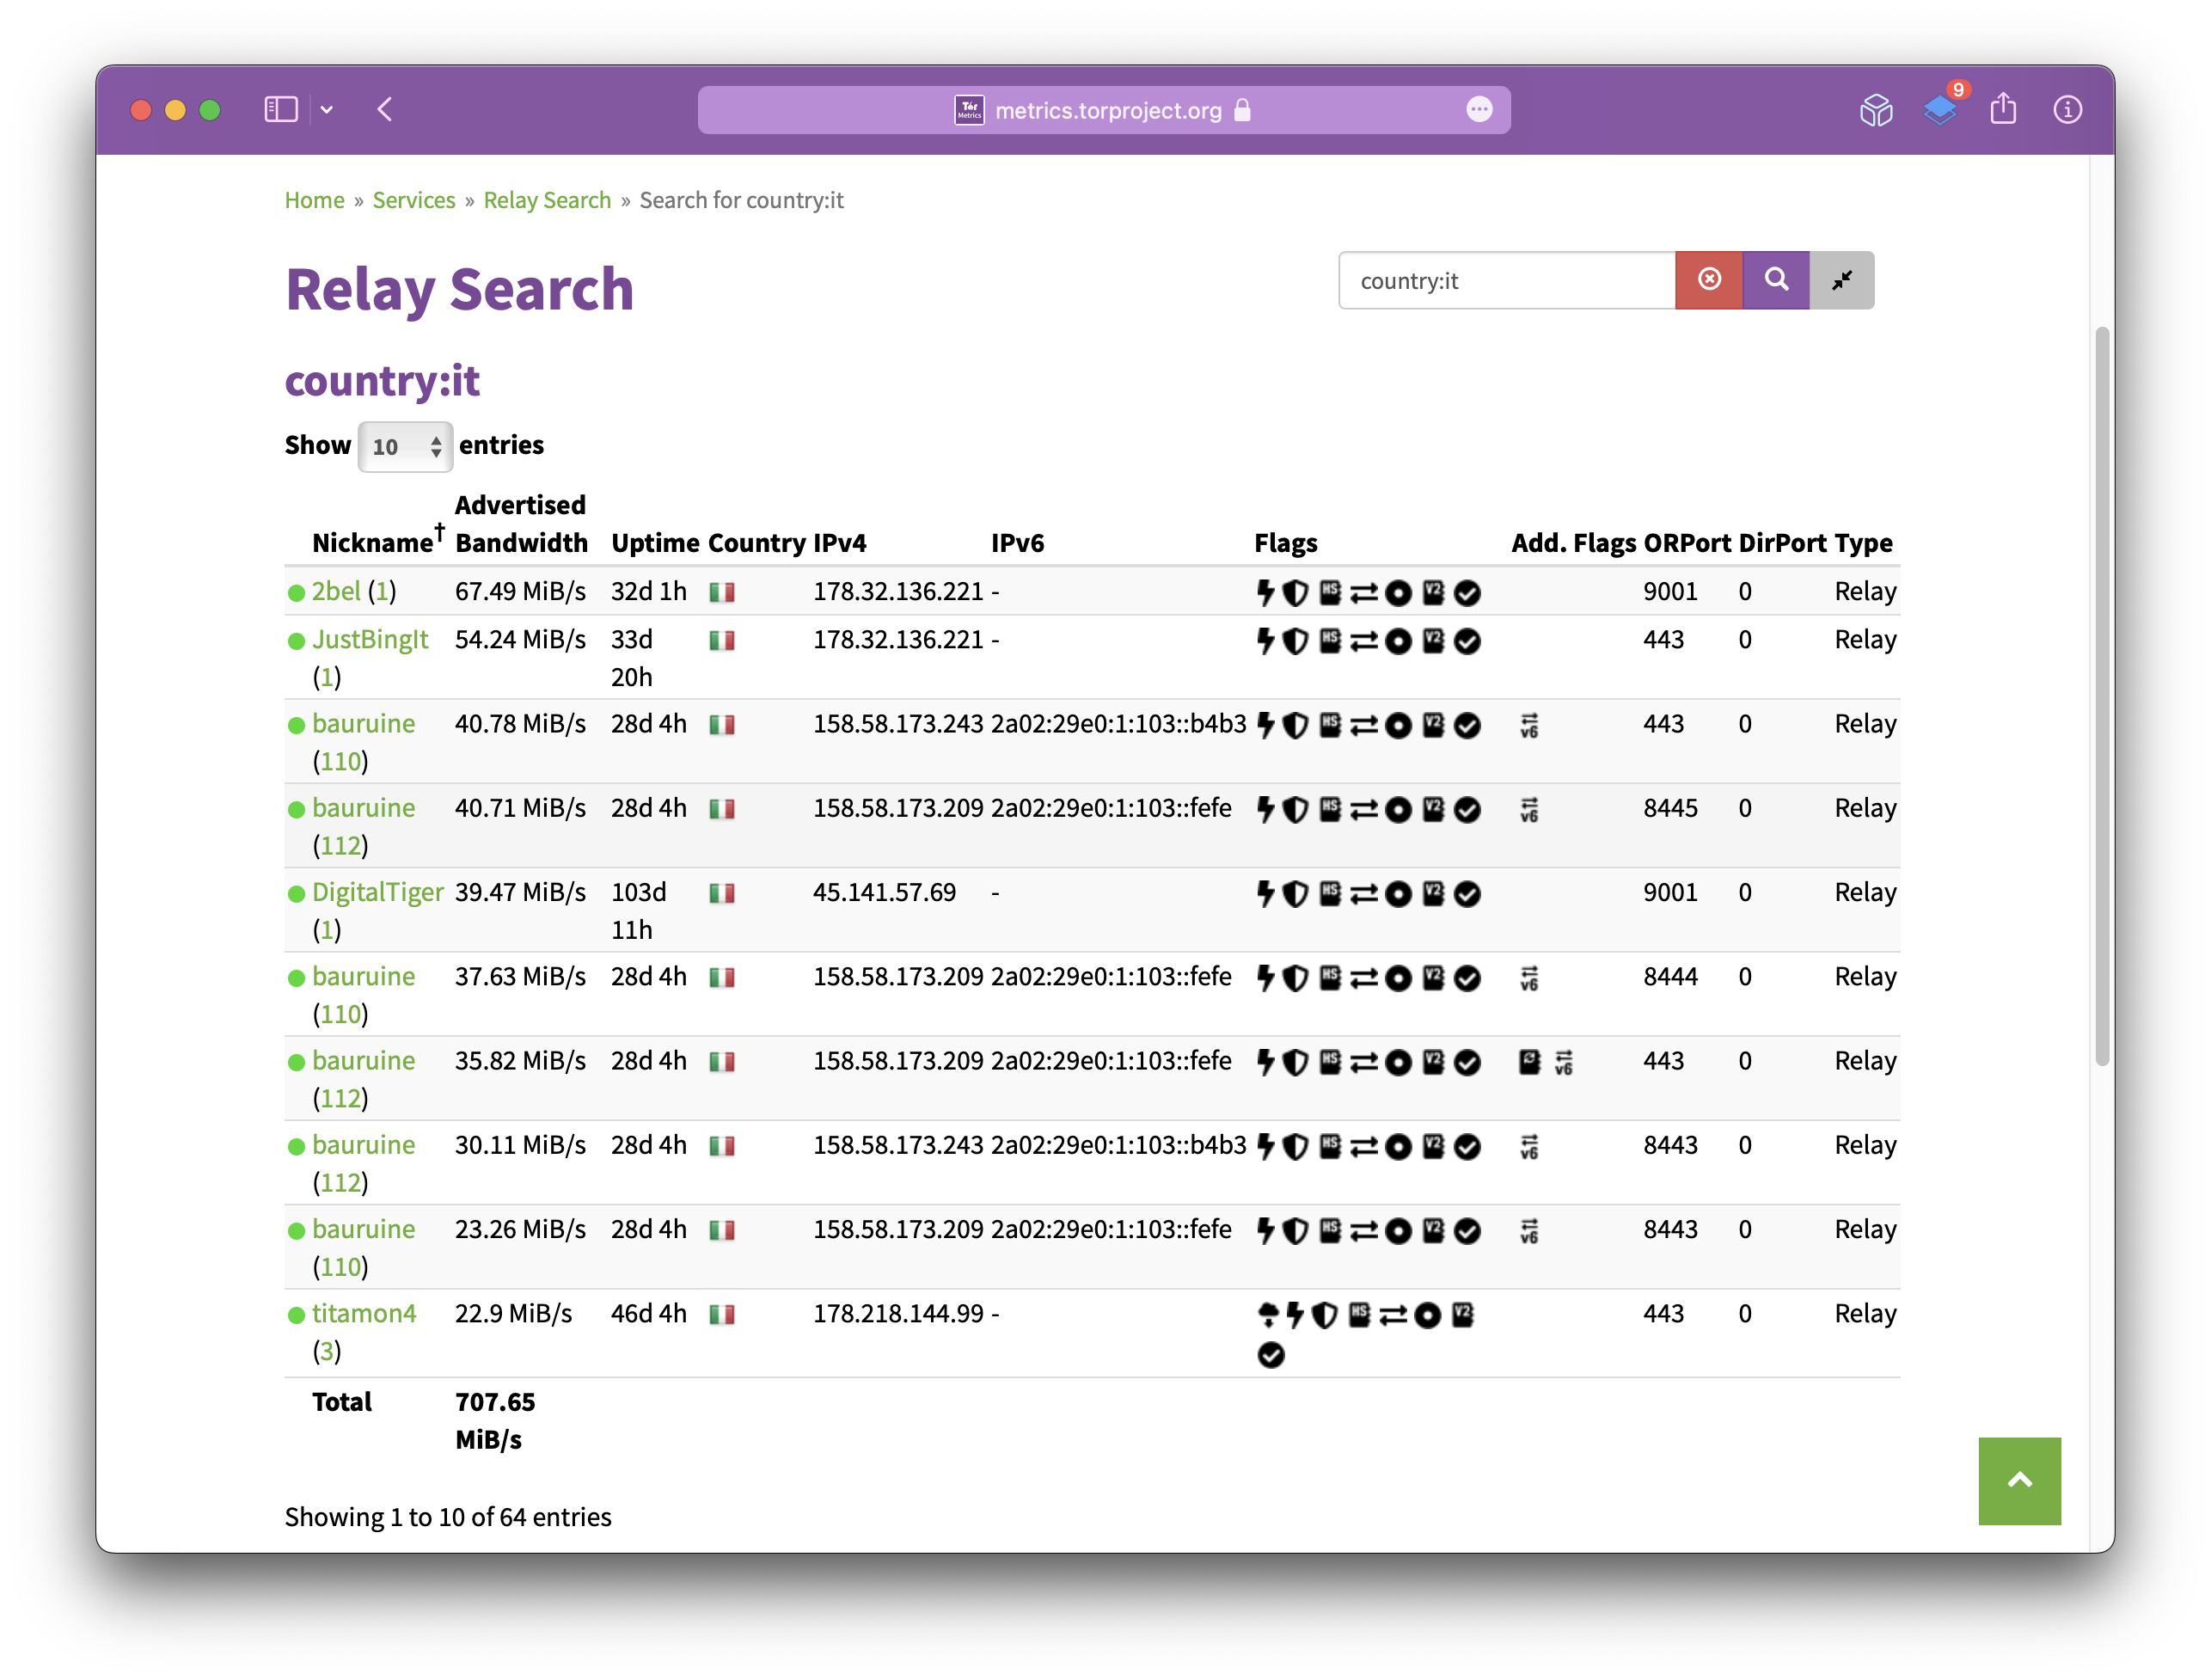
\includegraphics[width=\textwidth]{TorRelays}
    \caption{Statistiche dei Tor Relay in Italia}
}

\newpage
\section{Directory Servers} \label{sec:DirectoryServers}
I directory server sono un piccolo sottogruppo di onion router utilizzati per tracciare i cambiamenti nella topologia di rete. 
In particolare un directory server agisce come un server HTTP accessibile dai client per ottenere lo stato della rete e la lista dei router aggiornata periodicamente dagli stessi OR. \\
Quando il directory server riceve un aggiornamento da un OR prima di tutto controlla la chiave d'identità del router, garantendo che un attaccante non possa fingersi un OR manomettendo la rete \cite{ChaumMixes}. 
Il software di accesso alla rete onion è precaricato con le informazioni sui directory server e le relative chiavi, le informazioni di rete vengono aggiornate periodicamente dall'OP. \\

I directory server sono anche fondamentali per la connessione agli onion services, infatti ogni servizio creato genera un \emph{Onion Service Descriptor} contenente una lista degli introduction points e la chiave pubblica, il pacchetto viene criptato con la chiave privata e inviato al directory server che quindi agisce come fosse un DNS server per gli onion services. 
Quando l'utente tenta la connessione a un sito onion richiede e riceve dal directory server il relativo \emph{Descriptor} per l'indirizzo onion, usa la chiave pubblica, derivata dalla stringa dell'indirizzo onion a cui vuole connettersi, per decriptare il pacchetto \\
Nel caso il Directory Server fosse compromesso e contenesse un Descriptor malevolo generato per reindirizzare il traffico\footnote{Che però non potrà avere la stessa chiave privata}, l'indirizzo onion che possediamo non sarebbe in grado\footnote{tramite la chiave pubblica al suo interno nascosta} di decriptare le informazioni, dato che sono state criptate con una differente chiave privata
\cite{OnionServicesOverview}.
Non c'è neanche la necessità di determinare se le informazioni sono correte, perché a patto che la chiave privata non sia resa pubblica, nessuno potrà manomettere il Descriptor senza renderlo illeggibile e/o \emph{"indecifrabile"}
\section{Tor Browser}
Una delle principali vulnerabilità della rete Tor è la possibilità che un servizio web crei un codice JavaScript\footnote{che viene eseguito sul browser dell'utente} malevolo in grado di ottenere informazioni sull'indirizzo dell'utente deanonimizzandolo. 
Gli sviluppatori di Tor Browser hanno inserito appositamente un sistema di sicurezza che blocca gli script, questo però di contro porta molti siti a non funzionare correttamente. \\
Essendo la rete Tor fortemente basata sulla criptografia la navigazione di un sito onion tramite Tor non fa comparire alcun avviso di sicurezza in caso di mancanza di HTTPS, dato che il traffico è già criptato. 
Da tenere inoltre in considerazione che un certificato proveniente da una Certificate Authority potrebbe generare problemi di anonimizzazione del servizio a causa della Certificate Transparency\cite{CertificateTransparency} \\
\newpage
\section{Dimostrazione da Wireshark}

Ci sono diversi elementi che possono indicare l'esistenza di un circuito onion, innanzitutto esso viene creato sfruttando il protocollo TLS\footnote{In particolare la nuova versione di Tor usa TLSv1.3} tramite TCP, inserendo quindi TLS come filtro in Wireshark possiamo vedere i pacchetti con cui viene generato il circuito.
\importImage{
    \label{fig:Wireshark_circuit_raw}
    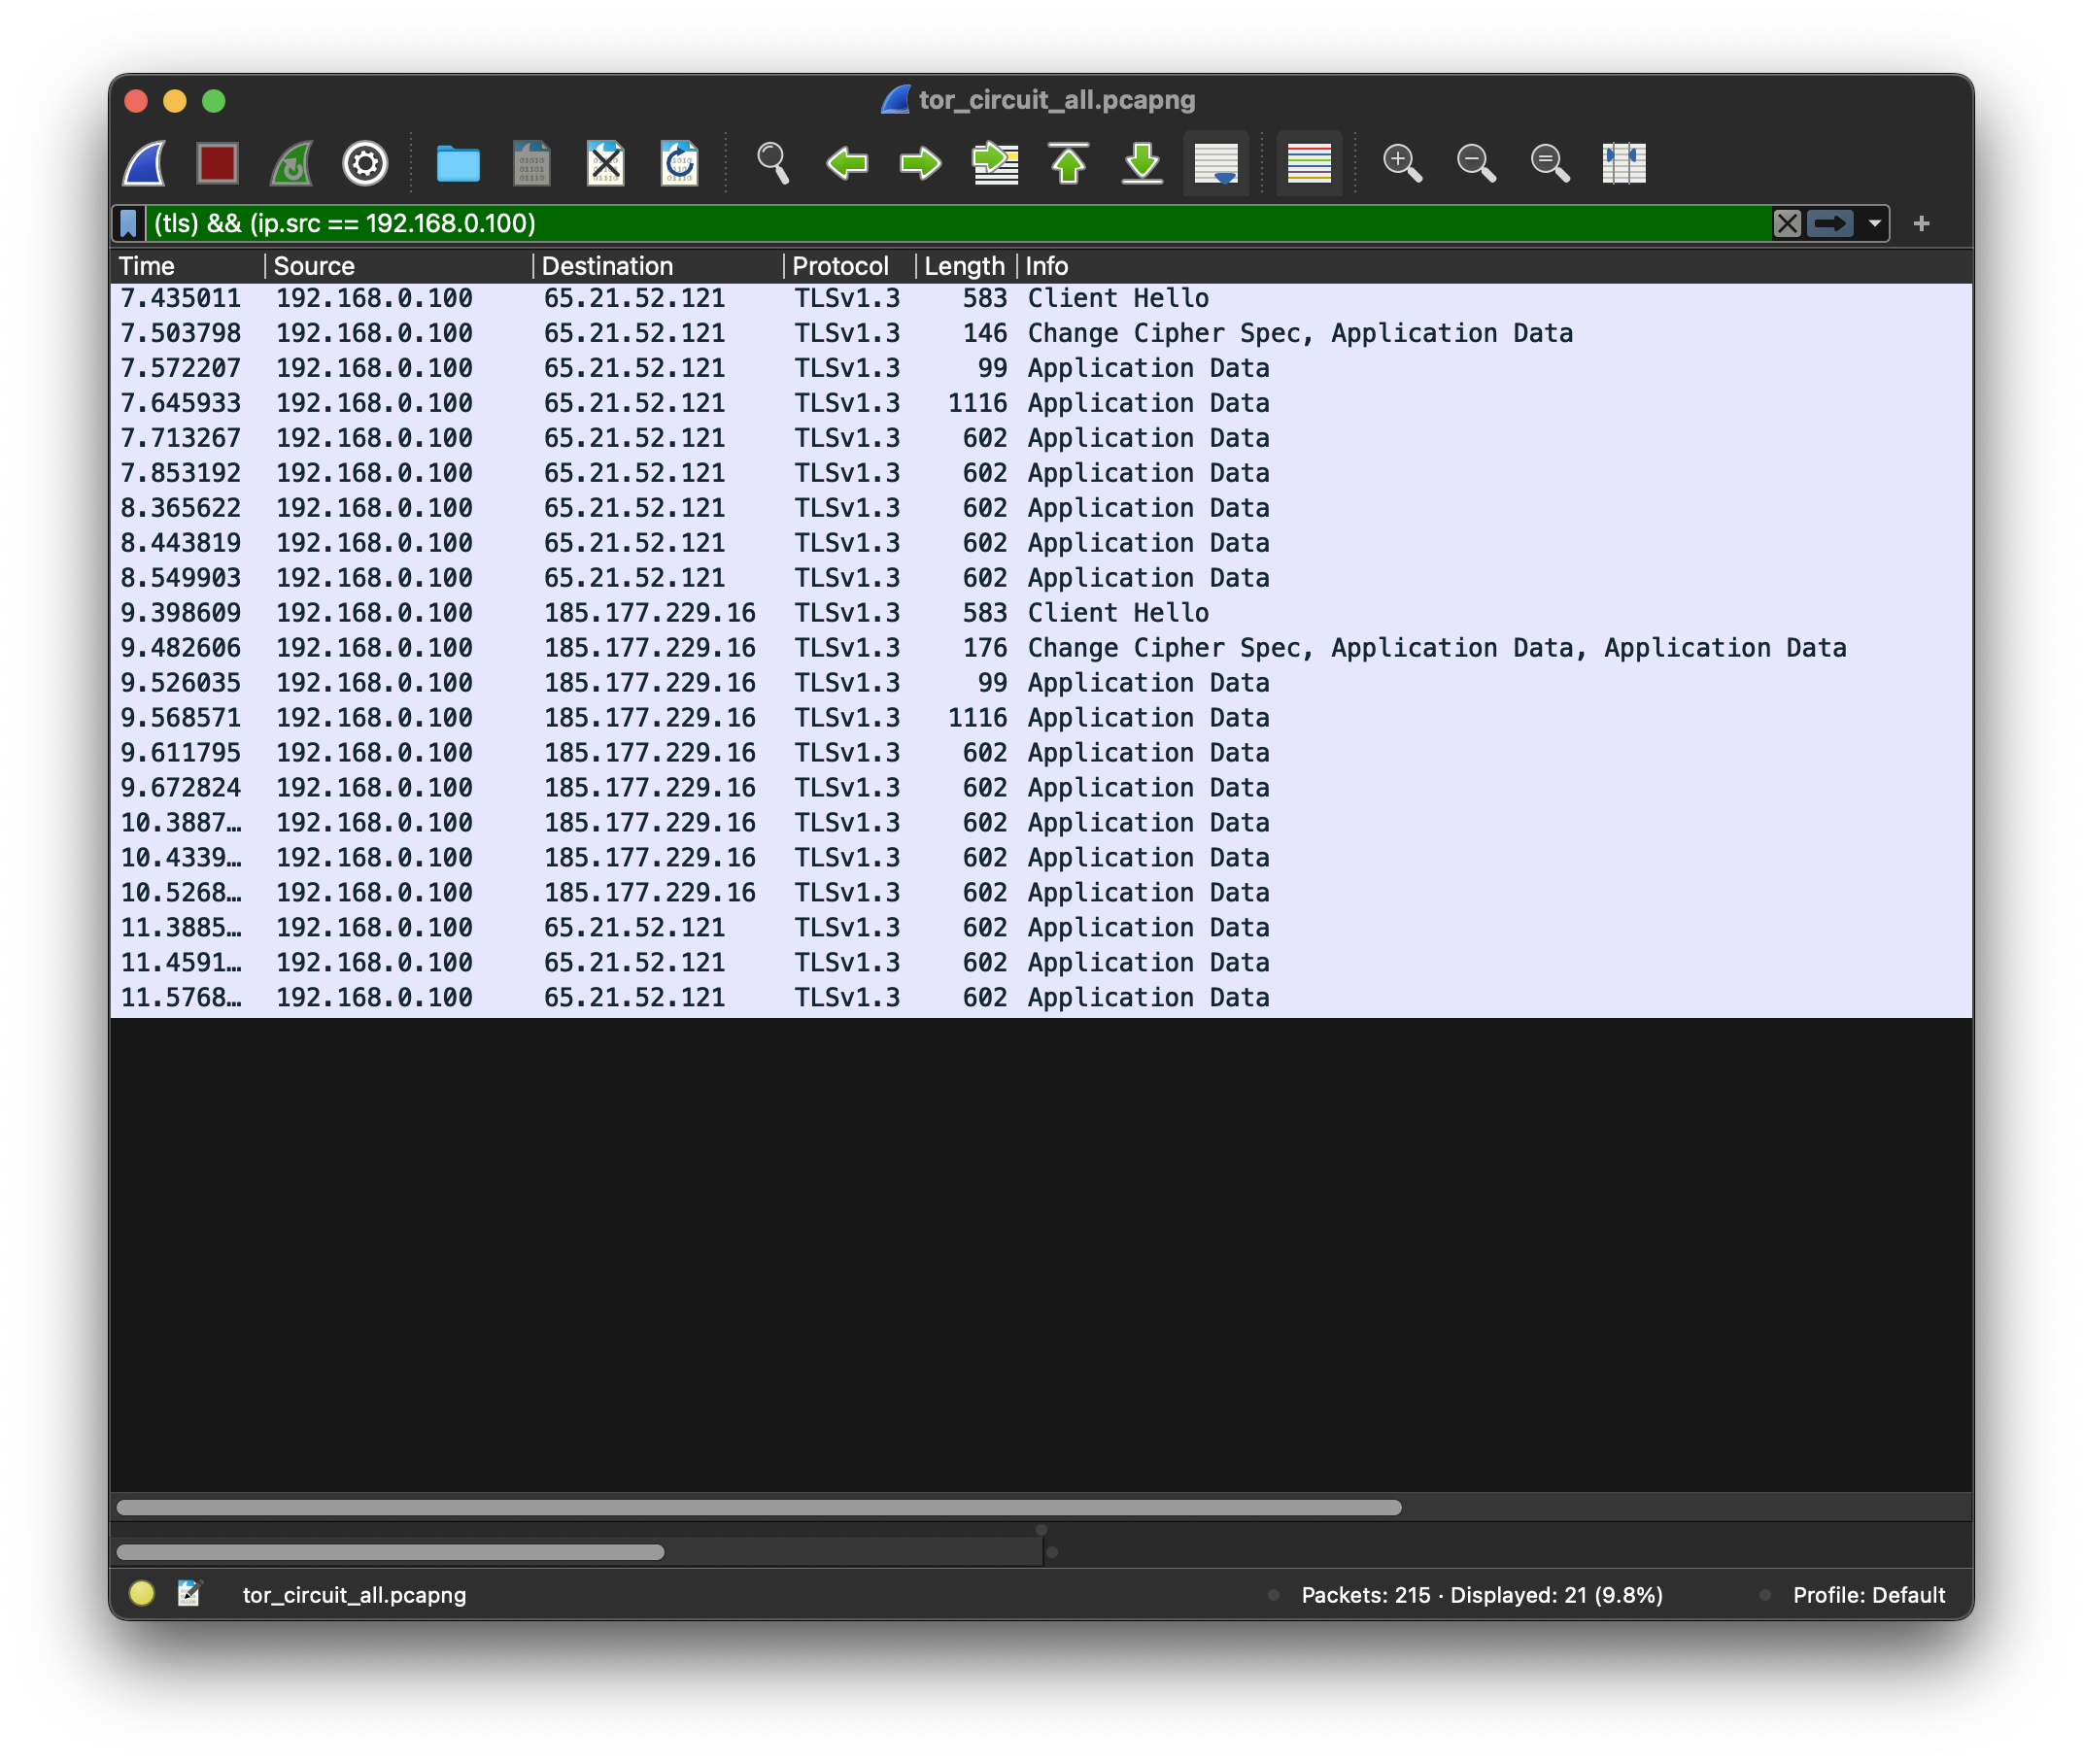
\includegraphics[width=\textwidth]{Wireshark/circuit_raw}
    \caption{Wireshark circuit}
}\\
Da qui vediamo che i due IP principali a cui il dispositivo si connette sono \lstinline{65.21.52.121} e \lstinline{185.177.229.16}. Vediamo anche che Tor scambia con questi due IP lo stesso numero e tipo di pacchetti con la stessa quantità di byte, per cui vi è una correlazione.
Eseguendo il filtro per IP possiamo quindi vedere tutti i pacchetti che i due dispositivi si scambiano
\newpage
\importImage{
    \label{fig:Wireshark_IP_Filtering}
    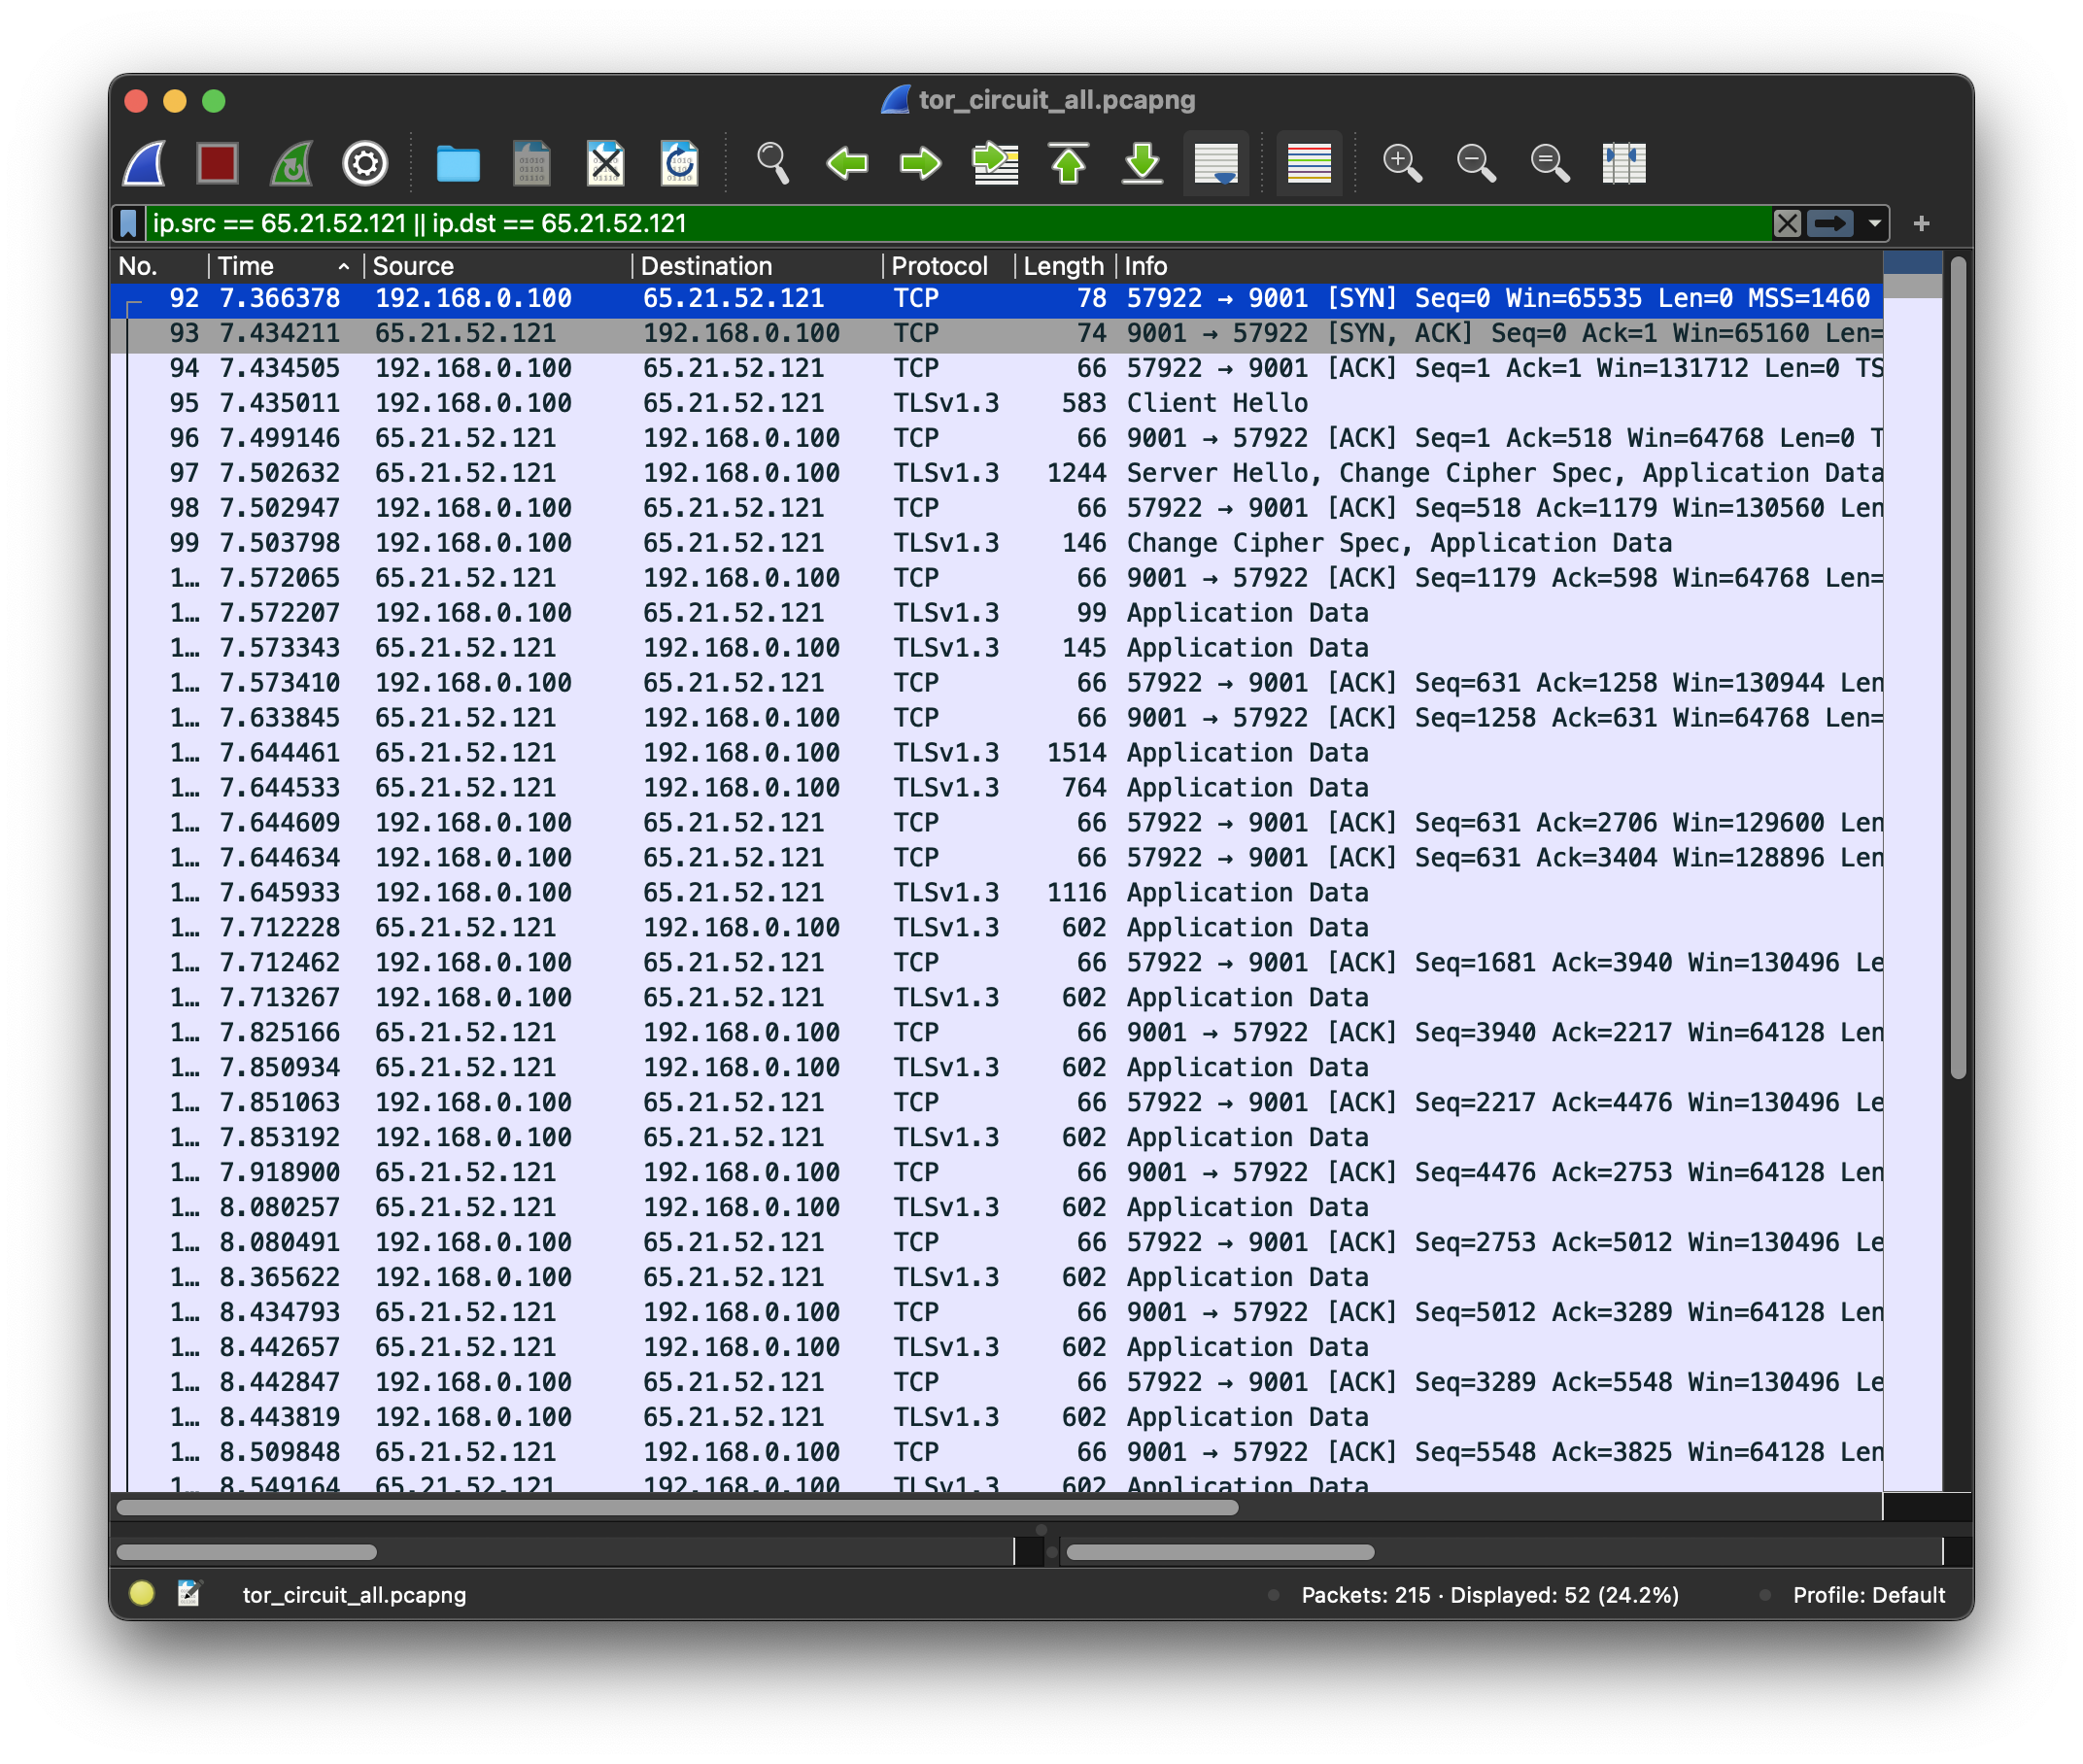
\includegraphics[width=\textwidth]{Wireshark/IP_Filtering}
    \caption{Wireshark IP filtering}
}
Vediamo quindi che inizialmente viene eseguito un TCP handshake, successivamente inizia lo scambio di chiavi tramite TLSv1.3, possiamo inoltre notare che la porta con cui comunichiamo con il server \lstinline{65.21.52.121} è la 9001\footnote{Tor Project suggerisce di non usare la porta 9001 per i bridge relay perché è facilmente associabile alla rete Onion\cite{OnionAvoid9001}}.
A ogni messaggio TLS corrisponde una risposta ACK TCP che possiamo ignorare.
\newpage
Analizziamo il primo pacchetto TLS che viene inviato al server, è denominato \textbf{Client Hello} e possiede vari campi
\begin{itemize}
    \item \textbf{Cipher Suites}, una lista di protocolli di criptografia simmetrica supportati dal client che invia la richiesta\cite{RFC8448}. In questo caso i protocolli supportati sono 18, tra cui abbiamo \lstinline{AES 128 GCM SHA256} e \lstinline{AES 256 GCM SHA384}
    \item Compression Methods, implementato in TLSv1.3 solo per retro compatibilità dei server, che possono anche ricevere e gestire richieste TLSv1.2. A differenza dei client TLSv1.3 che devono impostare questo parametro a 0 (null), altrimenti riceveranno un \lstinline{illegal_parameter message}
    \item \textbf{Extensions}, usato sia dalle applicazioni che sfruttano TLS, come onion, che da alcune funzionalità di TLSv1.3, implementate come estensioni per mantenere la retro compatibilità. In tal modo i server legacy possono semplicemente ignorare le estensioni non riconosciute
\end{itemize}
\cite{TLSv1_3}
\importImage{
    \label{fig:Client_Hello}
    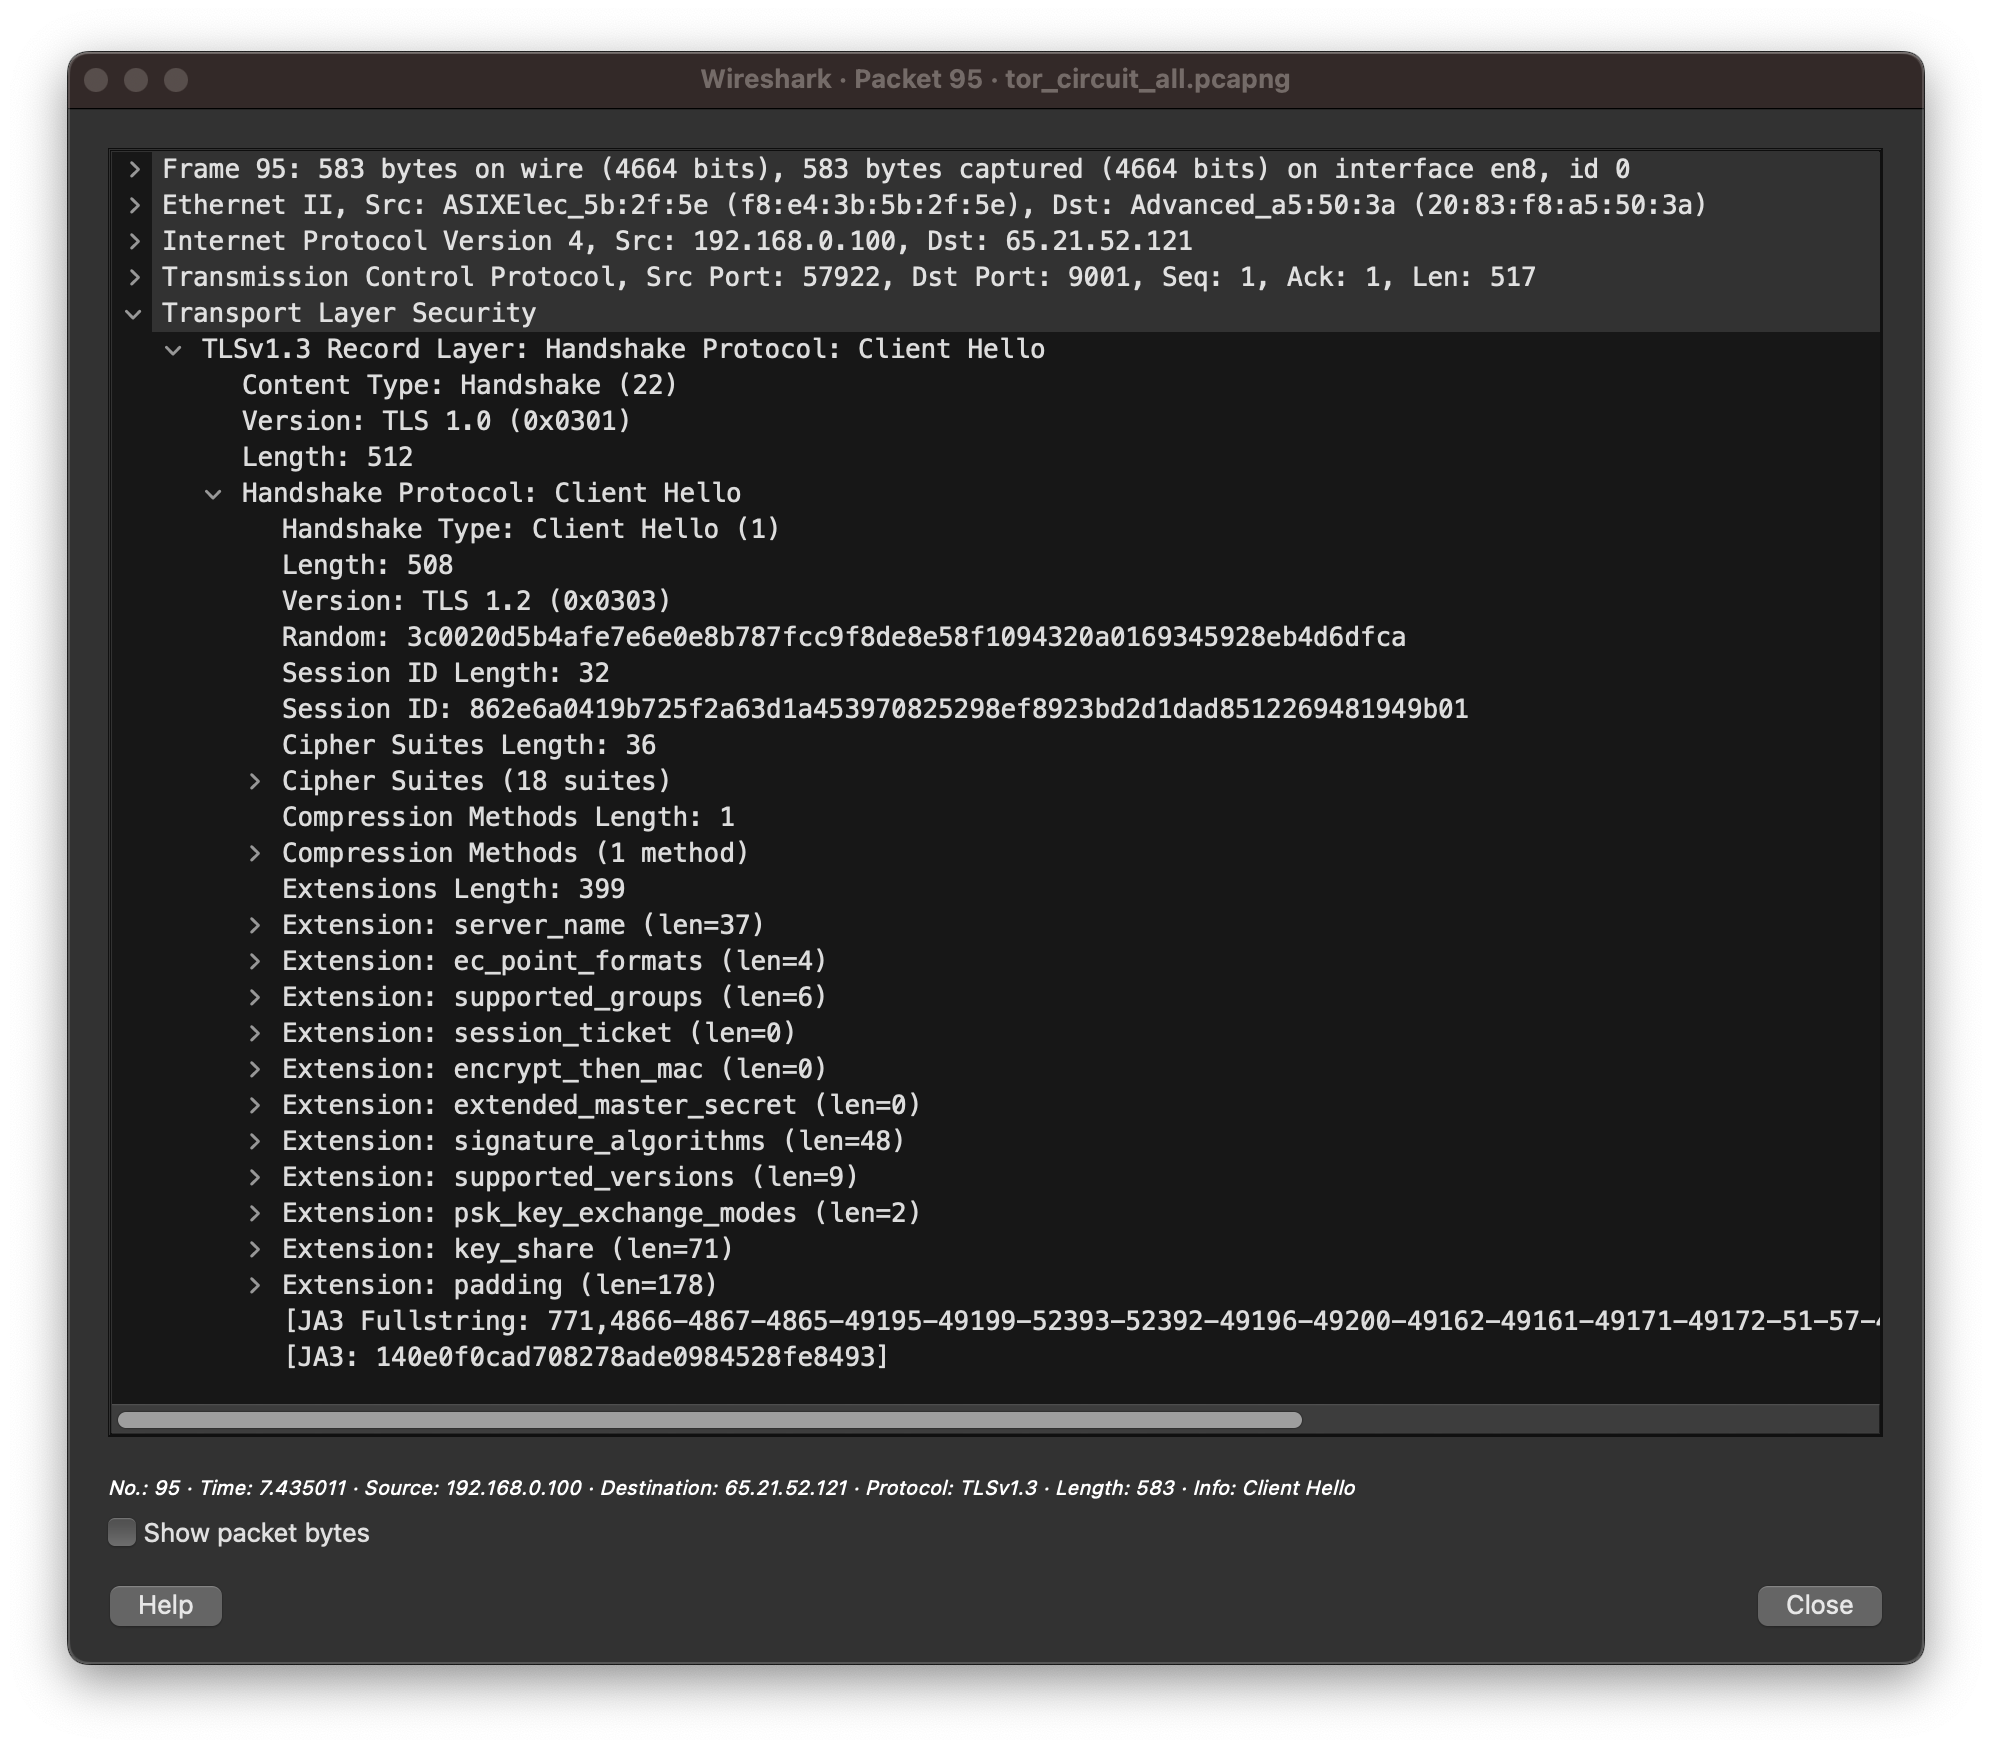
\includegraphics[width=\textwidth]{Wireshark/Client_Hello}
    \caption{Client Hello}
}
\newpage
Come vediamo onion sfrutta diverse estensioni
\begin{itemize}
    \item \lstinline{server_name}, utilizzato per facilitare le connessioni sicure, indica il nome del server\cite{RFC6066}
    \item \lstinline{ec_point_formats}, sta per Elliptic Curve Point Formats e indica i formati di compressione(Point Formats) supportati dal client\cite{RFC8422}
    \item \lstinline{supported_groups}, precedentemente chiamato Supported Elliptic Curves Extensions, indica gli Elliptic Curves utilizzati ordinati in base alla preferenza del client \cite{RFC8422}
    \item \lstinline{session_ticket}, non usato
    \item \lstinline{encrypt_then_mac}, non usato
    \item \lstinline{extended_master_secret}, non viene più usato ma deve comunque essere indicato per retro compatibilità\cite{RFC7627}
    \item \lstinline{signature_algorithms}, utilizzato per indicare gli algoritmi di firma supportati dal client\cite{RFC8446}
    \item \lstinline{supported_versions}, utilizzato dal client per indicare le versioni di TLS supportate e dal server per indicare la versione utilizzata \cite{RFC8446}
    \item \lstinline{psk_key_exchange_modes}, utilizzato esclusivamente dal client per indicare le modalità di condivisione della passkey\cite{RFC8446}
    \item \lstinline{key_share}, utilizzato per inviare la chiave pubblica con cui criptare il traffico del server verso questo client, indicando anche il tipo di chiave\cite{RFC8446}
    \item \lstinline{padding}, utilizzato come una sequenza di 0 sufficienti per far raggiungere al pacchetto almeno 512 bytes di lunghezza. Il campo può essere omesso per i pacchetti di almeno 512 bytes. Con pacchetti di lunghezza tra 509 e 511 bytes questo campo porta il pacchetto a superare i 512 bytes, in quanto non può essere inferiore ai 4 bytes\cite{RFC7685}
\end{itemize}
\newpage
Successivamente il server risponde con un \textbf{Server Hello}, indicando un unico cipher suite e le estensioni \lstinline{supported_versions} e \lstinline{key_share}.
\importImage{
    \label{fig:Server_Hello}
    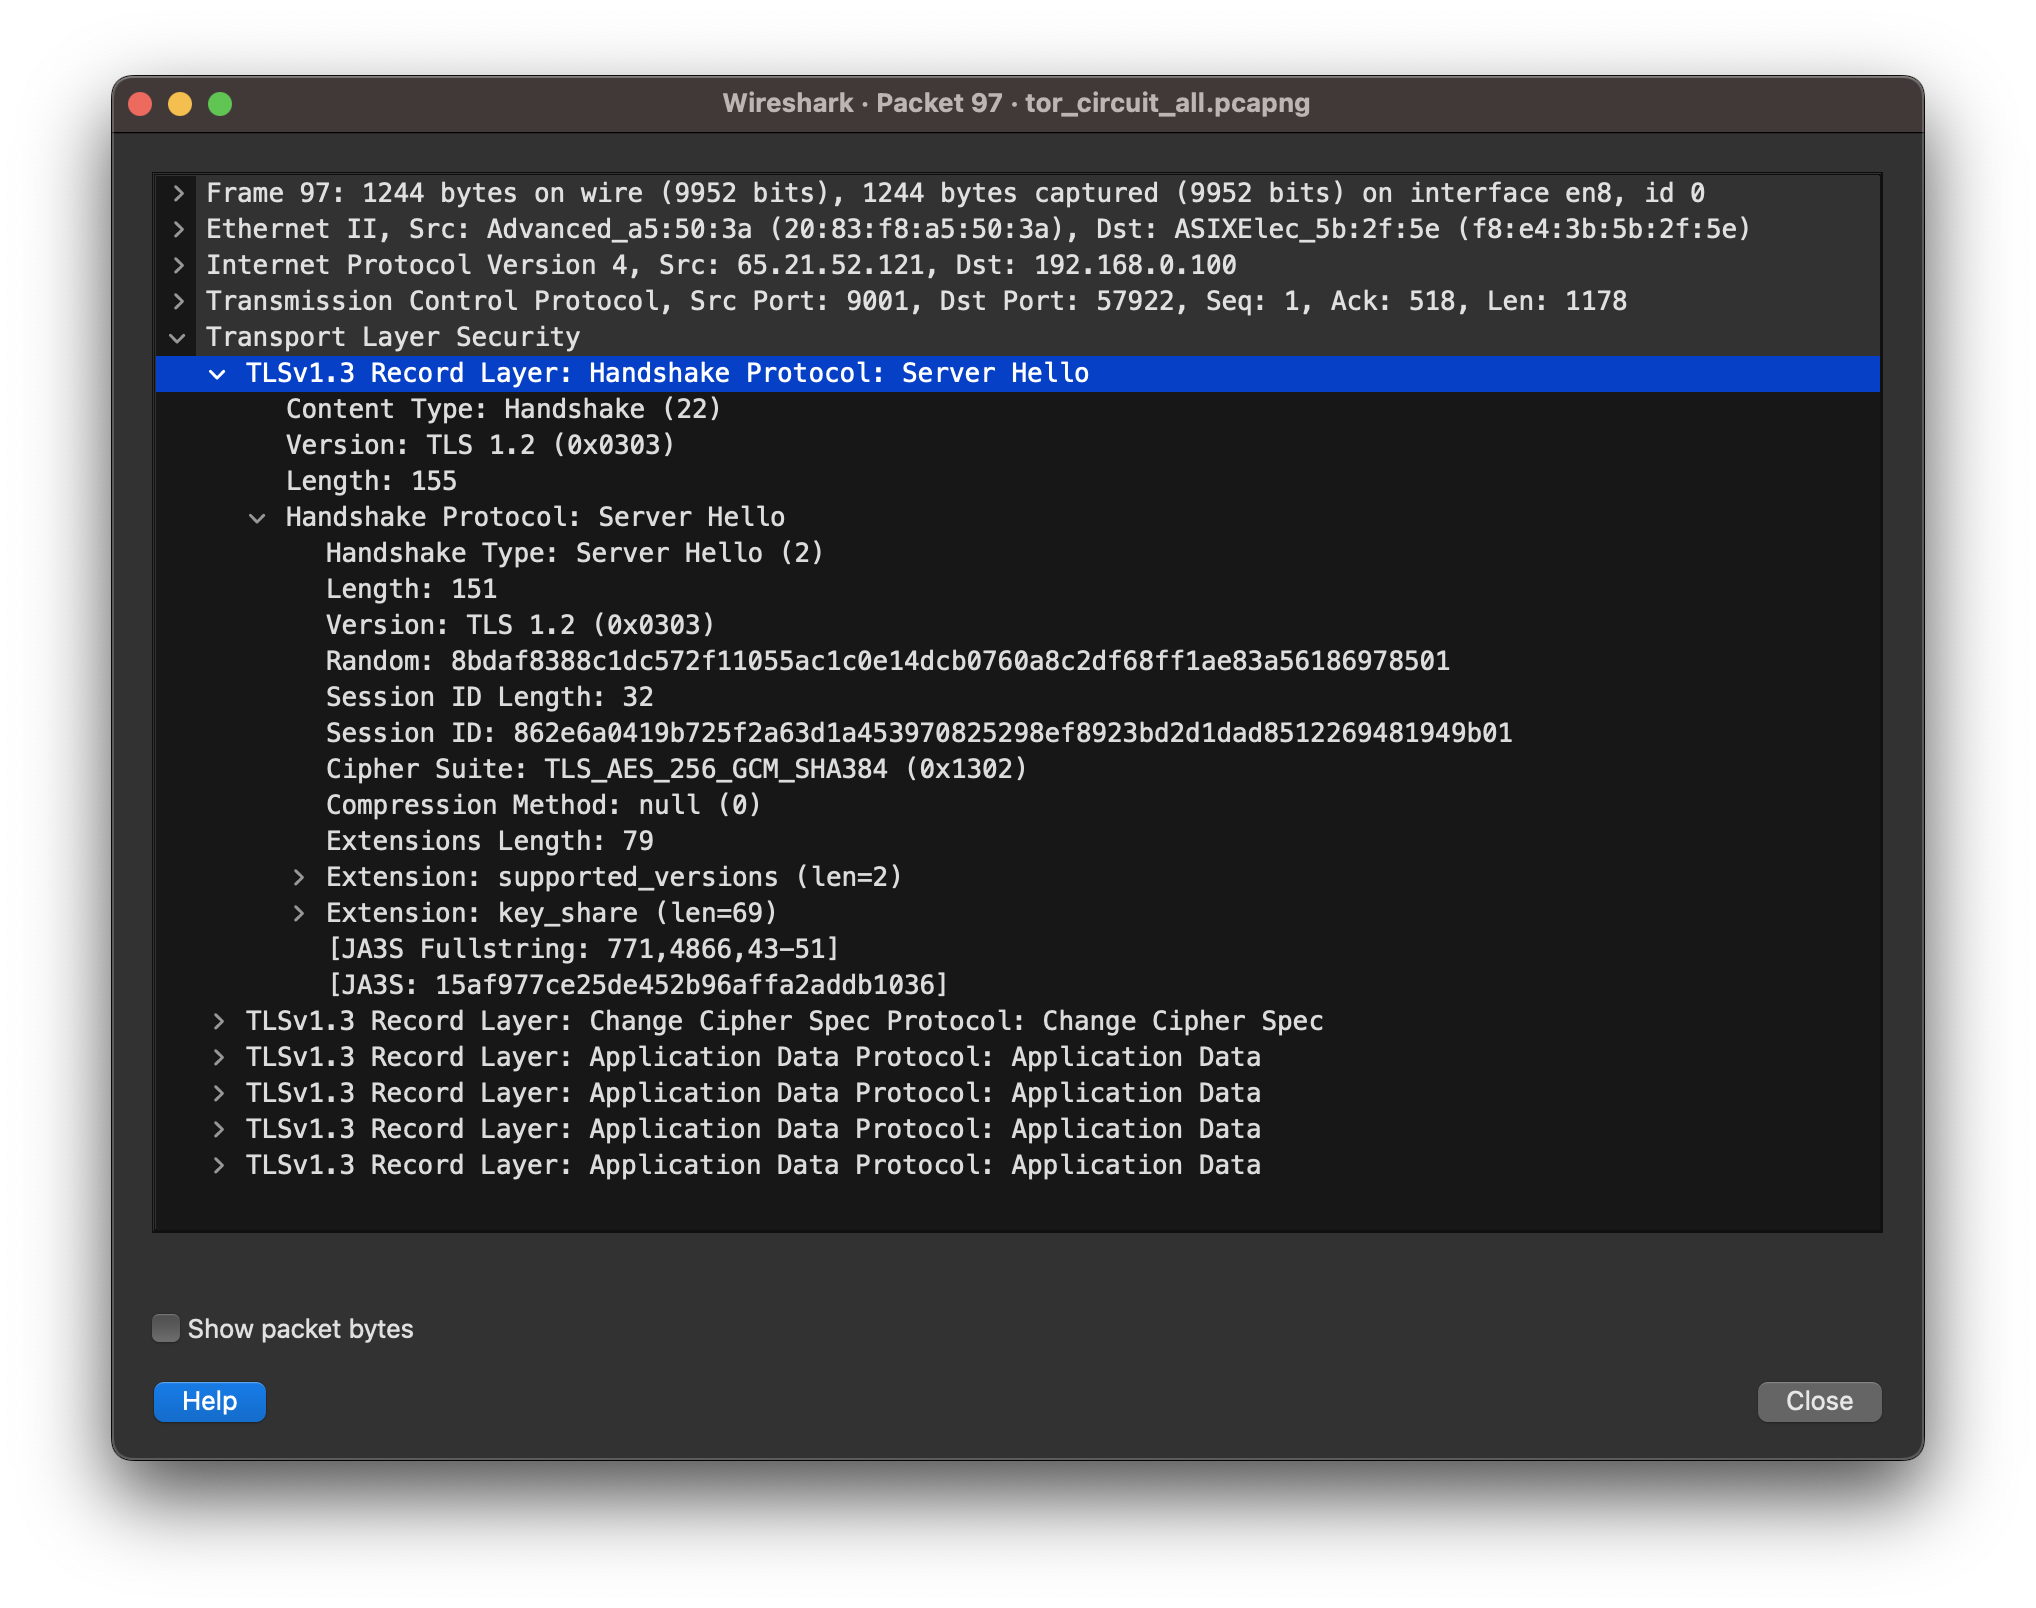
\includegraphics[width=\textwidth]{Wireshark/Server_Hello}
    \caption{Server Hello e Application Data}
}\\
Da qui la connessione viaggia per il circuito onion e tutti i dati sono criptati con le chiavi che possiede solo il client Tor, per cui non è possibile analizzare il traffico, possiamo solo intuire quali pacchetti sono destinati alla rete onion.


% \section{Vulnerabilità} % Qui si parla delle vulnerabilità di onion v2 per cui si è passati a v3

    \chapter{Implementazione}

\section{Servizi Onion}
Nelle comuni reti internet i servizi vengono utilizzati facendo richie basate sugli indirizzi IP pubblici, la sorgente e destinazione di un pacchetto è quindi conosciuta da tutti i dispositivi che la ricevono. 
Onion invece garantisce l'anonimato non solo ai clienti ma anche agli utenti che mettono a disposizione i server per fornire servizi, nascondendone l'indirizzo IP. 
Questo viene fatto tramite uno pseudonimo di lungo termine, identico in tutti i circuiti e stabile anche al un fallimento di un router \\
I principali obiettivi sono
\begin{itemize}
    \item Gli attaccanti non devono riuscire a manipolare la rete sostituendosi un servizio esistente. Questo livello di affidabilità deriva dalla criptografia asimmetrica che ci garantisce che il servizio a cui cerchiamo di connetterci sia autentico, solo lui possiede la copia privata della chiave pubblica con cui tentiamo la connessione
    \item Sicurezza dagli attacchi DoS, viene fatto tramite l'uso di più punti d'ingresso alla rete 
\end{itemize}
La creazione di un servizio onion passa per diversi punti prima di poter essere raggiungibile
\begin{enumerate}
    \item Genera una coppia di chiave pubblica e privata per identificarsi
    \item Definisce alcuni onion router come punti di ingresso nella rete, da cui riceverà le richieste dei clienti e invia loro la chiave pubblica
    \item Crea un circuito con ogni punto di ingresso
    \item Invia al servizio di lookup onion le informazioni sui punti d'ingresso e l'hash della chiave pubblica che sarà usata come hostname
\end{enumerate}
Quando un utente tenta la connessione
\begin{enumerate}
    \item Inizialmente esegue il lookup del dominio
    \item Successivamente sceglie un OR come tramite per il servizio e genera un circuito verso di esso, sfruttando uno specifico cookie per identificare il servizio
    \item Viene generato uno stream verso uno dei punti d'ingresso del servizio con tutte le informazioni riguardo se stesso, il nodo tramite e il cookie. Tutto viene criptato con la chiave pubblica del servizio
    \item Inizia l'handshake di Diffle-Hellman tra OP e servizio
    \item Il servizio onion a sua volta genera un circuito verso il nodo tramite per poter rispondere all'OP con la seconda parte dell'handshake
    \item Il nodo tramite collega i due circuiti generando un circuito dati bidirezionale 
\end{enumerate}
Sia l'utente che il server non vengono modificati e il server non è nemmeno a corrente che il suo traffico viaggia per una rete onion \cite{ChaumMixes}
\section{Onion V3}

La terza generazione di onion nasce per risolvere alcuni problemi di sicurezza. In particolare rispetto alla seconda generazione
\begin{itemize}
    \item Vengono aggiornati i sistemi di crittografia, da SHA1/DH/RSA1024 a SHA3/ed25519/curve25519
    \item Vengono migliorati i directory server e il directory protocol
    \item Viene cambiato il sistema di hostname
\end{itemize}
Precedentemente venivano usati i primi 80 bit dell'hash (SHA1) della chiave pubblica per creare un'hostname, un esempio yyhws9optuwiwsns.onion, nella terza generazione vengono codificati in base32
\begin{itemize}
    \item La chiave pubblica, un totale di 32 byte in ed25519
    \item Il checksum di 2 byte
    \item Un byte di versione, di default '\textbackslash x03' 
\end{itemize}
In totale il nuovo hostname possiede 56 caratteri \cite{Torv3} \\
Un esempio è l'indirizzo \emph{pg6mmjiyjmcrsslvykfwnntlaru7p5svn6y2ymmju6nubxndf4pscryd.onion}, una volta decriptato sfruttando il base32 definito nell' RFC 3548 e 4648 abbiamo la seguente stringa 79bcc625184b05194975c28b66b66b0469f7f6556fb1ac3189a79b40dda32f1f214703, come notiamo termina con 03, il byte di versione
\section{Studio delle tecnologie}

Per creare un servizio sulla rete onion si possono usare una moltitudine di tecnologie differenti, ogni singolo aspetto necessita di effettuare delle scelte. \\
\begin{itemize}
    \item Deploy del Server, la prima scelta ricade sulla creazione del server e in particolare scegliere dove eseguire il deploy, ci sono molteplici motivi per usare un servizio cloud, tra cui la sicurezza e la facilità d'uso. Ci sono 3 principali competitor e molti altri secondari che per la maggior parte sfruttano i server di queste 3 aziende
    \begin{itemize}
        \item Microsoft Azure
        \item Google Cloud
        \item Amazon Web Service, il più importante servizio cloud, è gestito e reso disponibile da Amazon e possiede molti servizi tra cui scegliere. Per questa implementazione useremo il servizio EC2 messo a disposizione da AWS in una macchina t3.micro
    \end{itemize}
    \item SO, la seconda scelta ricade sul sistema operativo della nostra macchina. Debian in particolare ha molti vantaggi, tra cui 
    \begin{itemize}
        \item Leggerezza, affidabilità e sicurezza derivate da un sistema GNU/Linux
        \item Maggiore utilizzo in ambienti server
        \item Nessun costo aggiuntivo derivato dall'aquisto di una licenza d'uso come Windows server
    \end{itemize}
    Useremo in particolare la versione 11
    \item Web Server, abbiamo due web server principali 
    \begin{itemize}
        \item Apache httpd, il più vecchio dei due, rilasciato con licenza Apache 2.0
        \item Nginx, un web server più moderno che fornisce diversi altri strumenti oltre al web server, tra cui il proxy e load balancer, è gratuito e come httpd è open source, ha superato apache da un paio di anni. Viene anche utilizzato in container docker, ma noi lo useremo in una classica macchina virtuale.
    \end{itemize}
\end{itemize}



\newpage
\section{Creazione del servizio}

Una volta creato l'account AWS possiamo creare una macchina virtuale andando nella sezione EC2 -> Instances -> Launch Instances, durante la configurazione possiamo selezionare le opzioni che abbiamo precedentemente analizzato
\begin{enumerate}
    \item Il nome
    \item Il sistema operativo da usare, selezioniamo Debian 11 e in particolare l'architettura x86,
    \item L'istanza scelta è una semplice t3.micro con 2 vCPU e 1 GiB di memoria
    \item Una coppia di due chiavi pubblica e privata, selezioniamo o creiamo una 
    \item Successivamente è fondamentale aggiungere alla macchina i giusti security group, di default AWS non consente nessun tipo di traffico in entrata o in uscita dalla macchina
    \begin{itemize}
        \item Consentire la connessione ssh alla porta 22
        \begin{figure}[h]
            \centering
            
\includegraphics[width=\textwidth]{securityGroup1}
            \caption{security Group 1, ssh in entrata}
            \label{fig:sec1}
        \end{figure}
        
        \item Consentire il traffico TCP in uscita
        \begin{figure}[h]
            \centering
            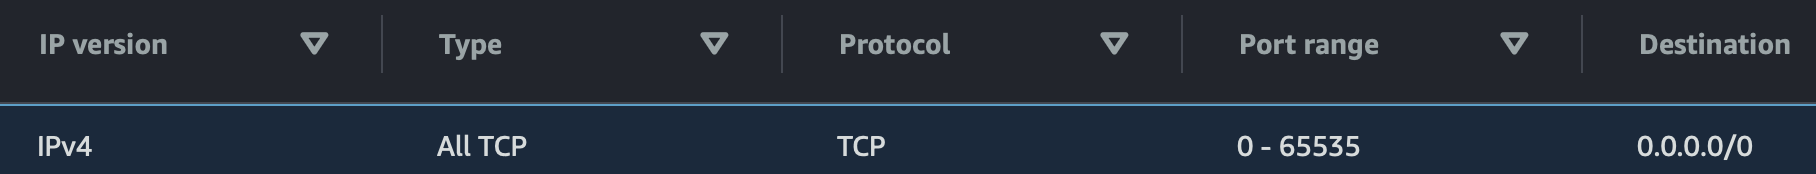
\includegraphics[width=\textwidth]{securityGroup2}
            \caption{security Group 2, TCP in uscita}
            \label{fig:sec2}
        \end{figure}
    \end{itemize}
\end{enumerate}


Una volta creata la macchina avremo la possibilità di scaricare la chiave privata con formato *.pem che useremo per connetterci tramite ssh alla shell della macchina
% [caption=connessione ssh]
% \lstinline{}
\begin{lstlisting}
    ssh -i key.pem admin@*.compute.amazonaws.com
\end{lstlisting}

La primissima operazione sarà l'aggiornamento dei repository e del sistema
% [caption=aggiornamento sistema]
\begin{lstlisting}
    sudo apt update && sudo apt full-upgrade -y
\end{lstlisting}

Poi installiamo il web server nginx che abbiamo analizzato prima
%[caption=Installazione Nginx]
\begin{lstlisting}
    sudo apt install nginx
\end{lstlisting}

Una volta completata l'installazione il web server è già avviato e in ascolto sulla porta 80 \\

Per installare tor è innanzitutto necessario installare \textbf{apt-transport-https} per utilizzare i repository tramite https
\begin{lstlisting}
    sudo apt install apt-transport-https
\end{lstlisting}
Poi aggiungiamo i repository TOR nella cartella \lstinline{/etc/apt/sources.list.d} \\
Dal comando \lstinline{lsb_release -c} possiamo vedere la distribuzione corrente e inserire il repository corretto nella configurazione, con Debian 11 siamo su di una distrubuzione bullseye, creiamo un file chiamato tor.list \footnote{Il nome è configurabile} con le seguenti righe
\begin{lstlisting}
    deb [signed-by=/usr/share/keyrings/tor-archive-keyring.gpg] https://deb.torproject.org/torproject.org bullseye main
    deb-src [signed-by=/usr/share/keyrings/tor-archive-keyring.gpg] https://deb.torproject.org/torproject.org bullseye main
\end{lstlisting}
Assicuriamoci che gpg sia installato nel sistema prima di aggiungere le chiavi
\begin{lstlisting}
    sudo apt install gpg
\end{lstlisting}
Aggiungiamo le chiavi gpg della repository appena creata
\begin{lstlisting}
    wget -qO- https://deb.torproject.org/torproject.org/A3C4F0F979CAA22CDBA8F512EE8CBC9E886DDD89.asc | gpg --dearmor | tee /usr/share/keyrings/tor-archive-keyring.gpg >/dev/null
\end{lstlisting}
Aggiorniamo gli index ed installiamo finalmente tor
\begin{lstlisting}
    sudo apt update && sudo apt install tor -y 
\end{lstlisting} \cite{TorRepo}
Generiamo il torrc file che ci servirà per impostare tutti i parametri di configurazione 
\begin{lstlisting}
    sudo tor -f /etc/tor/torrc
\end{lstlisting}
Apriamo il file e togliamo il commento alle righe \lstinline{HiddenServicePort 80 127.0.0.1:80} e \lstinline{HiddenServiceDir /var/lib/tor/hidden_service}, il primo indica che il traffico arrivato dalla porta virtuale (80) viene reindirizzato alla porta 80 del localhost, ovvero la porta in cui è in ascolto il web server nginx, il secondo ci serve per indicare la directory in cui si trova l'hostname del sito e le chiavi crittografiche. \\
Riavviamo tor per aggiornare la configurazione, assicurarci che il file torrc non contenga errori e che il sistema sia funzionante
% HiddenServiceDir /var/lib/tor/hidden_service/
\begin{lstlisting}
    sudo systemctl restart tor
\end{lstlisting}

\subsection{Gestire la comunicazione tramite i socket unix}

A questo punto tor ha creato gli introduction points e ha generato un circuito con ognuno di essi, ha generato le chiavi ed il proprio hostname, queste informazioni sono state aggiunte nella cartella che abbiamo inserito nell'HiddenServicePort, in particolare hostname contiene l'indirizzo tor del nostro servizio \cite{SetupOnionService} \\
Questo sistema però non è completamente sicuro, stiamo collegando tor con il web server tramite una porta, essendo entrambi i processi sulla stessa macchina il sistema ottimale è utilizzare un socket unix tra i due processi. Questo impedisce ad un utente non Tor di accedere direttamente al web server senza dover configurare firewall che comunque aggiungono complessità nella rete \\
Apriamo il file \lstinline{/etc/nginx/sites-enabled/default} e nella sezione server aggiungiamo il socket in ascolto, cosi che la comunicazione possa passare anche per il socket unix
\begin{lstlisting}
    listen unix:/var/run/website.sock;
\end{lstlisting}
Possiamo inoltre rimuovere la connessione dalla porta 80 commentando le seguenti righe
\begin{lstlisting}
    #listen 80 default_server;
    #listen [::]:80 default_server;
\end{lstlisting}
Dopo aver riavviato nginx ed esserci assicurati che non vi siano errori apriamo il file torrc e inseriamo lo stesso socket
\begin{lstlisting}
    HiddenServicePort 80 unix:/var/run/website.sock
\end{lstlisting}
Infine riavviamo tor, se tutto è andato a buon fine il servizio dovrebbe essere in grado di rispondere
\begin{lstlisting}
    sudo systemctl restart tor
\end{lstlisting}

\importImage{
    \label{fig:nginxConnection} 
    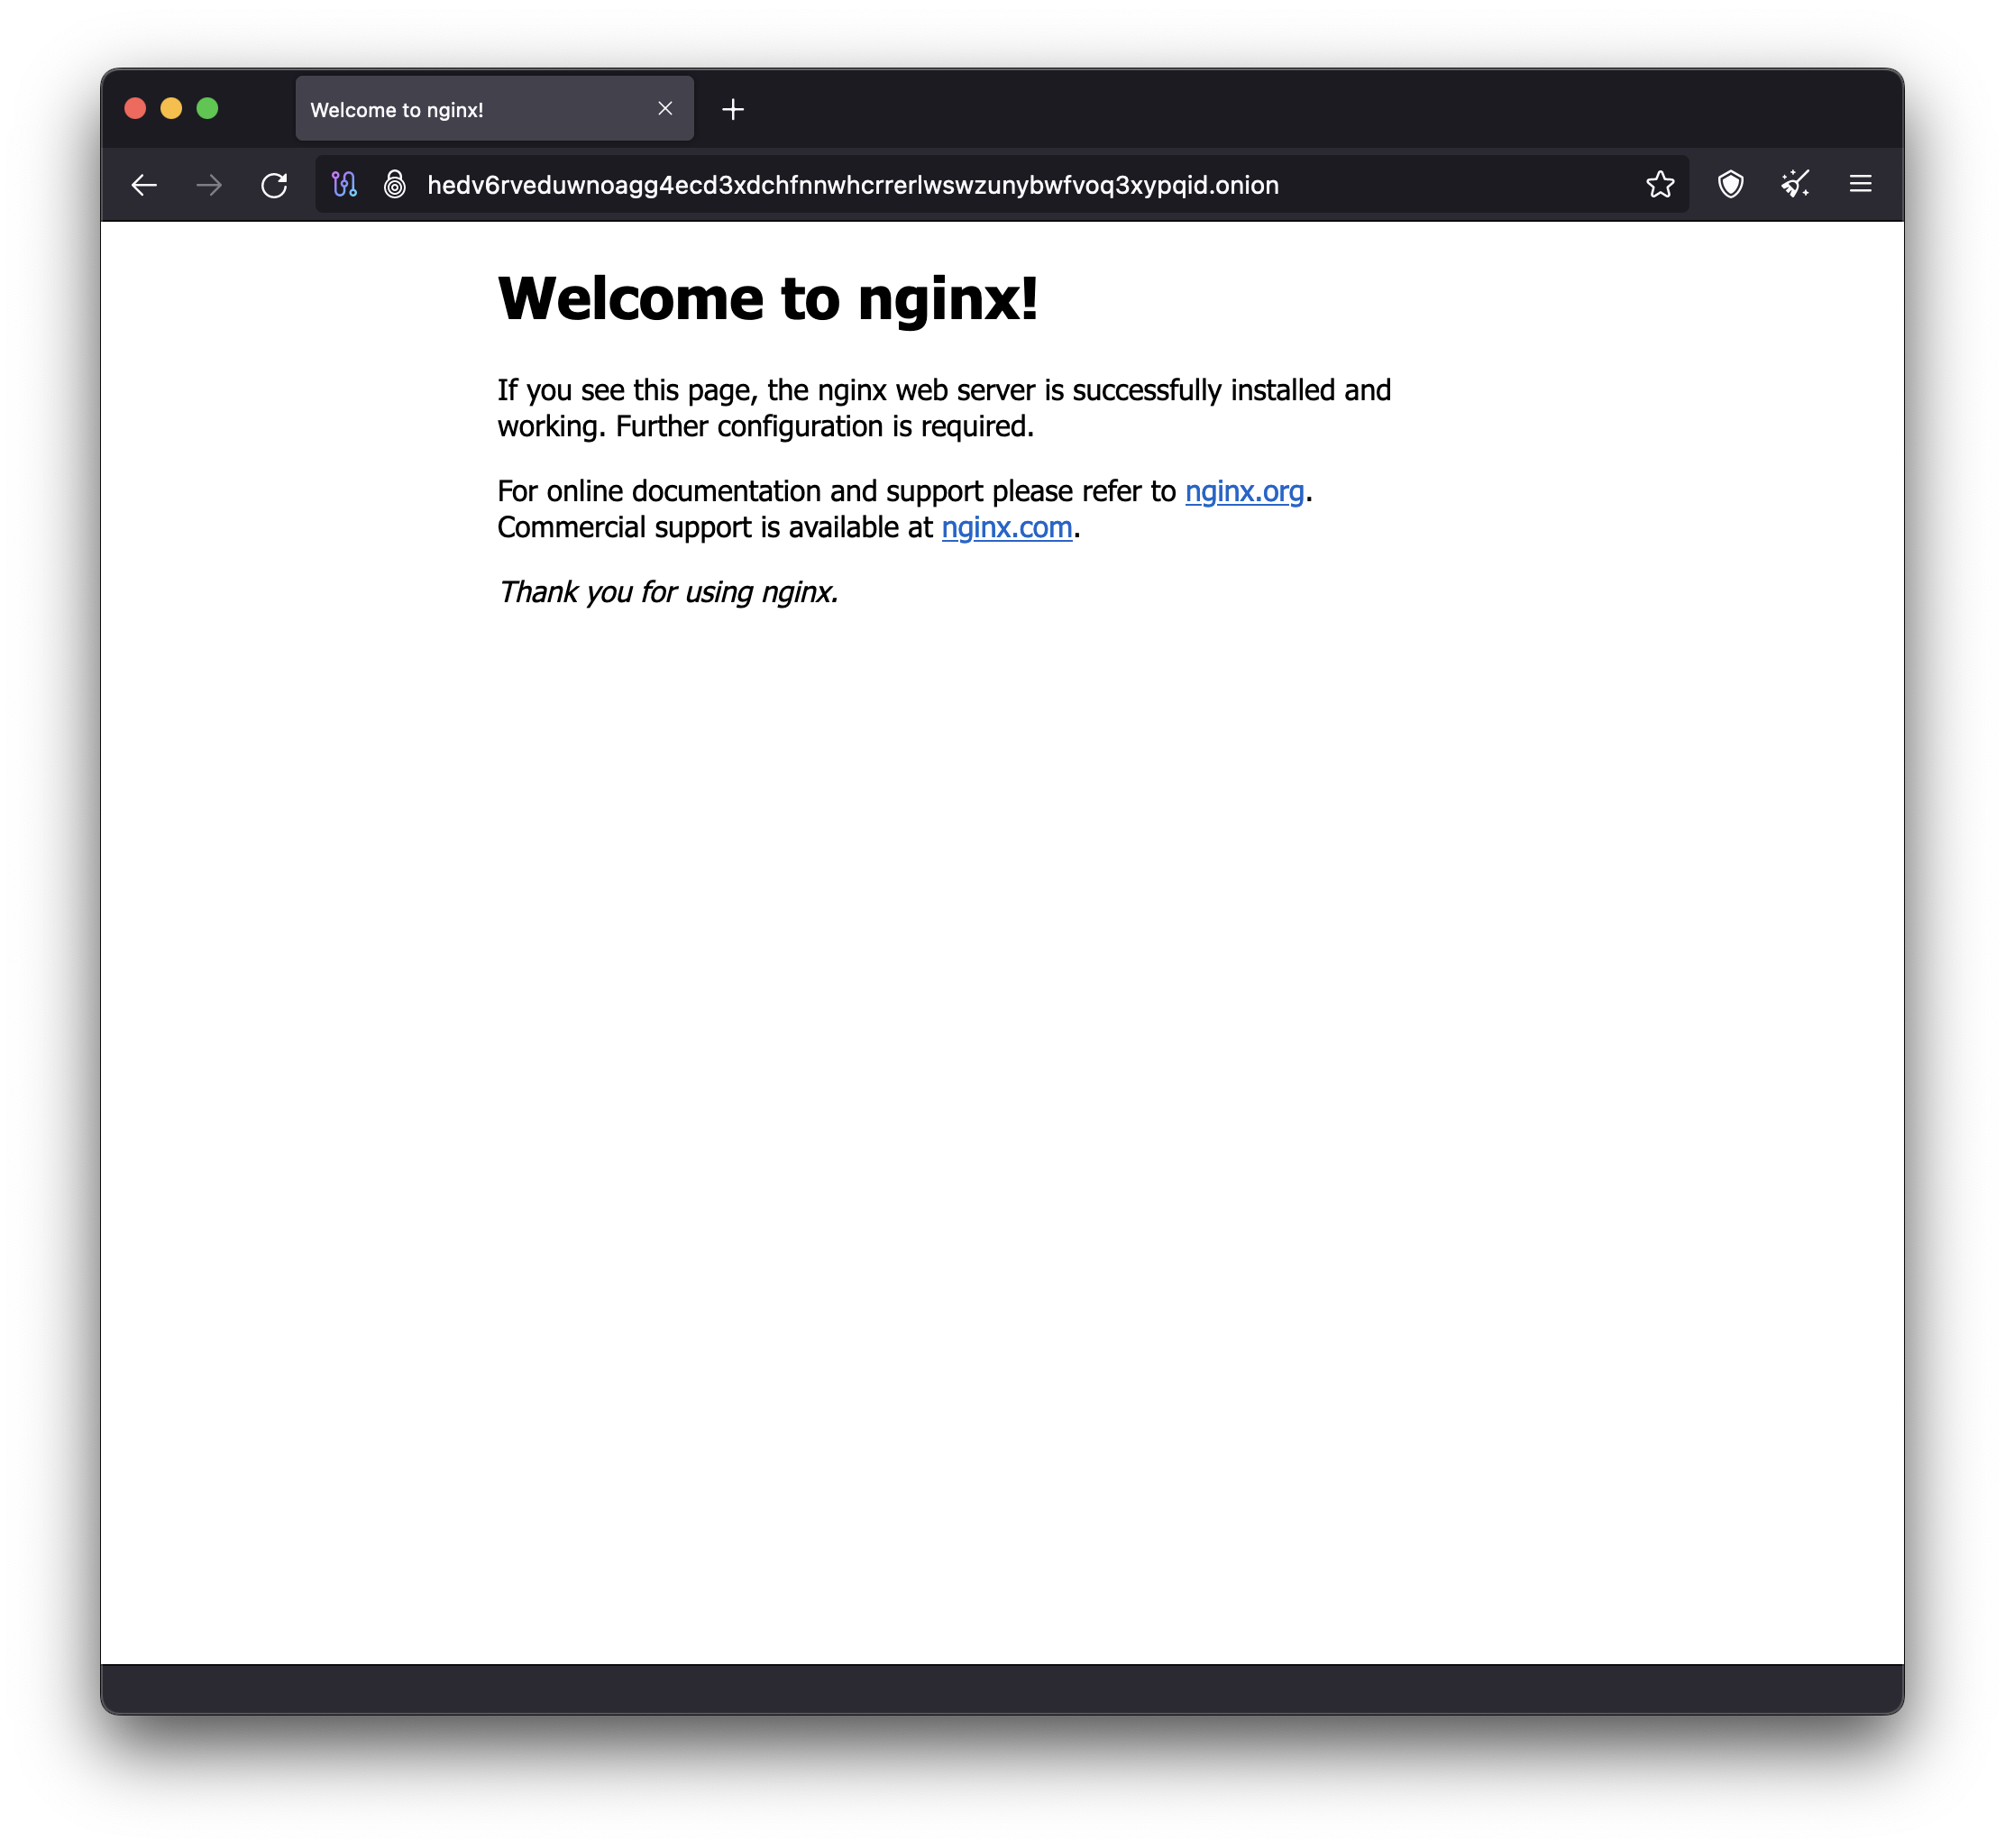
\includegraphics[width=\textwidth]{connectionSucceeded}
    \caption{Connessione al web server nginx}
}

\newpage
\subsection{Creazione di un url personalizzato}
Ora che il servizio è attivo e disponibile possiamo iniziare a configurarlo a nostro piacimento, la prima cosa che potremmo voler fare è cambiare l'hostname impostandone uno personalizzato, almeno in parte, un'esempio è il sito email di proton \textbf{protonmail}rmez3lotccipshtkleegetolb73fuirgj7r4o4vfu7ozyd.onion \\
Vi sono diversi strumenti per fare quest'operazione, si sfrutta la tecnica del brute force per generare chiavi ed indirizzi casuali fino a trovarne uno inizia con il termine che abbiamo scelto, potrebbe impiegare diverso tempo ed è consigliabile usare un computer più potente della nostra macchina virtuale. 
Per questa implementazione useremo il tool mkp224o \cite{V3AddressGeneratorRepo}, possiamo installarlo su linux o usarlo su windows da riga di comando semplicemente indicando il nome con cui dovrà iniziare

\footnote{Il file viene avviato direttamente dalla cartella del sorgente, per cui apponiamo \lstinline{./}}
\begin{lstlisting}
    ./mkp224o tesilm
\end{lstlisting}
    
Da notare che più caratteri si scelgono nel matching più il software impiegerà nella generazione di un dominio. Otteniamo il nuovo indirizzo del server\footnote{tesilm3jb64lw3upj4uu5fsxi2nrtbhbhkbu2dsbn46qka7j4kf7peqd.onion} con le relative chiavi \\
Possiamo copiarle sul server con scp usando l'opzione -i per definire il file d'identità, come facciamo con ssh
    
\begin{lstlisting}
    cd tesilm3jb64lw3upj4uu5fsxi2nrtbhbhkbu2dsbn46qka7j4kf7peqd.onion
    scp -i key.pem * admin@*.compute.amazonaws.com:~/var/lib/tor/hidden_service
\end{lstlisting}

Avviamo la connessione al server e riavviamo tor per impostare le modifiche

\importImage{
    \label{fig:mkpCommandOut} 
    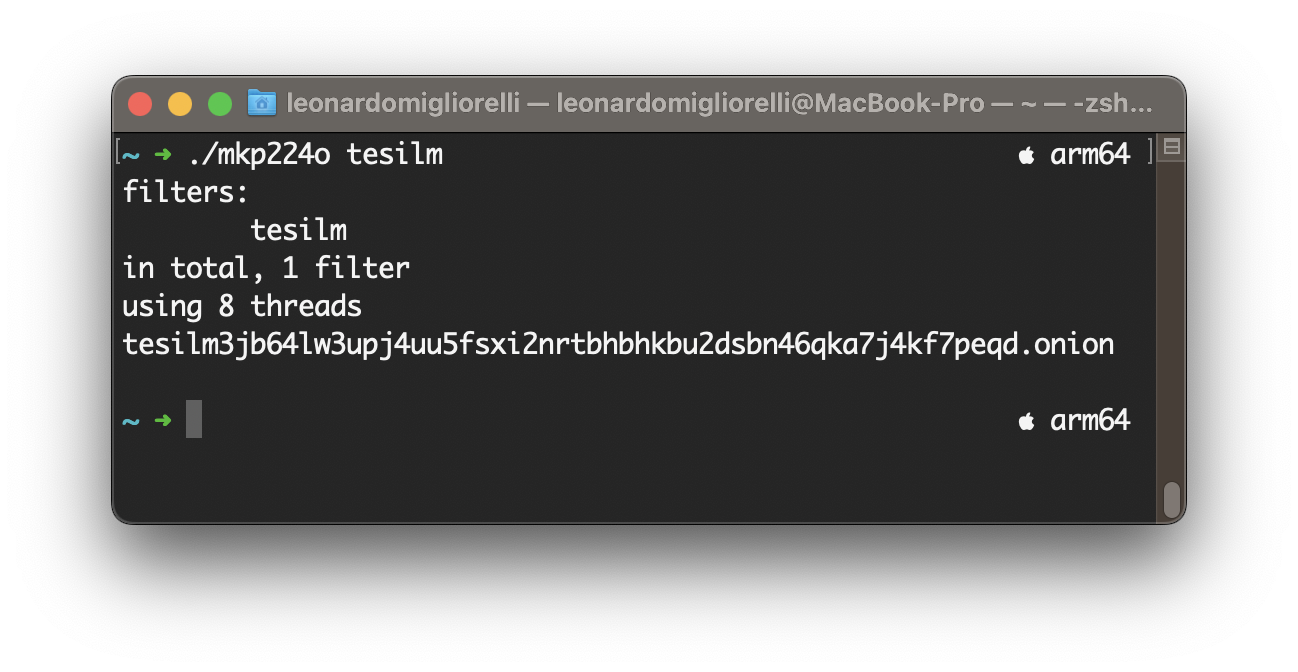
\includegraphics[width=\textwidth]{mkpCommandOut}
    \caption{Comando mkp224o e output}
}

\importImage{
    \label{fig:customAddressConnection} 
    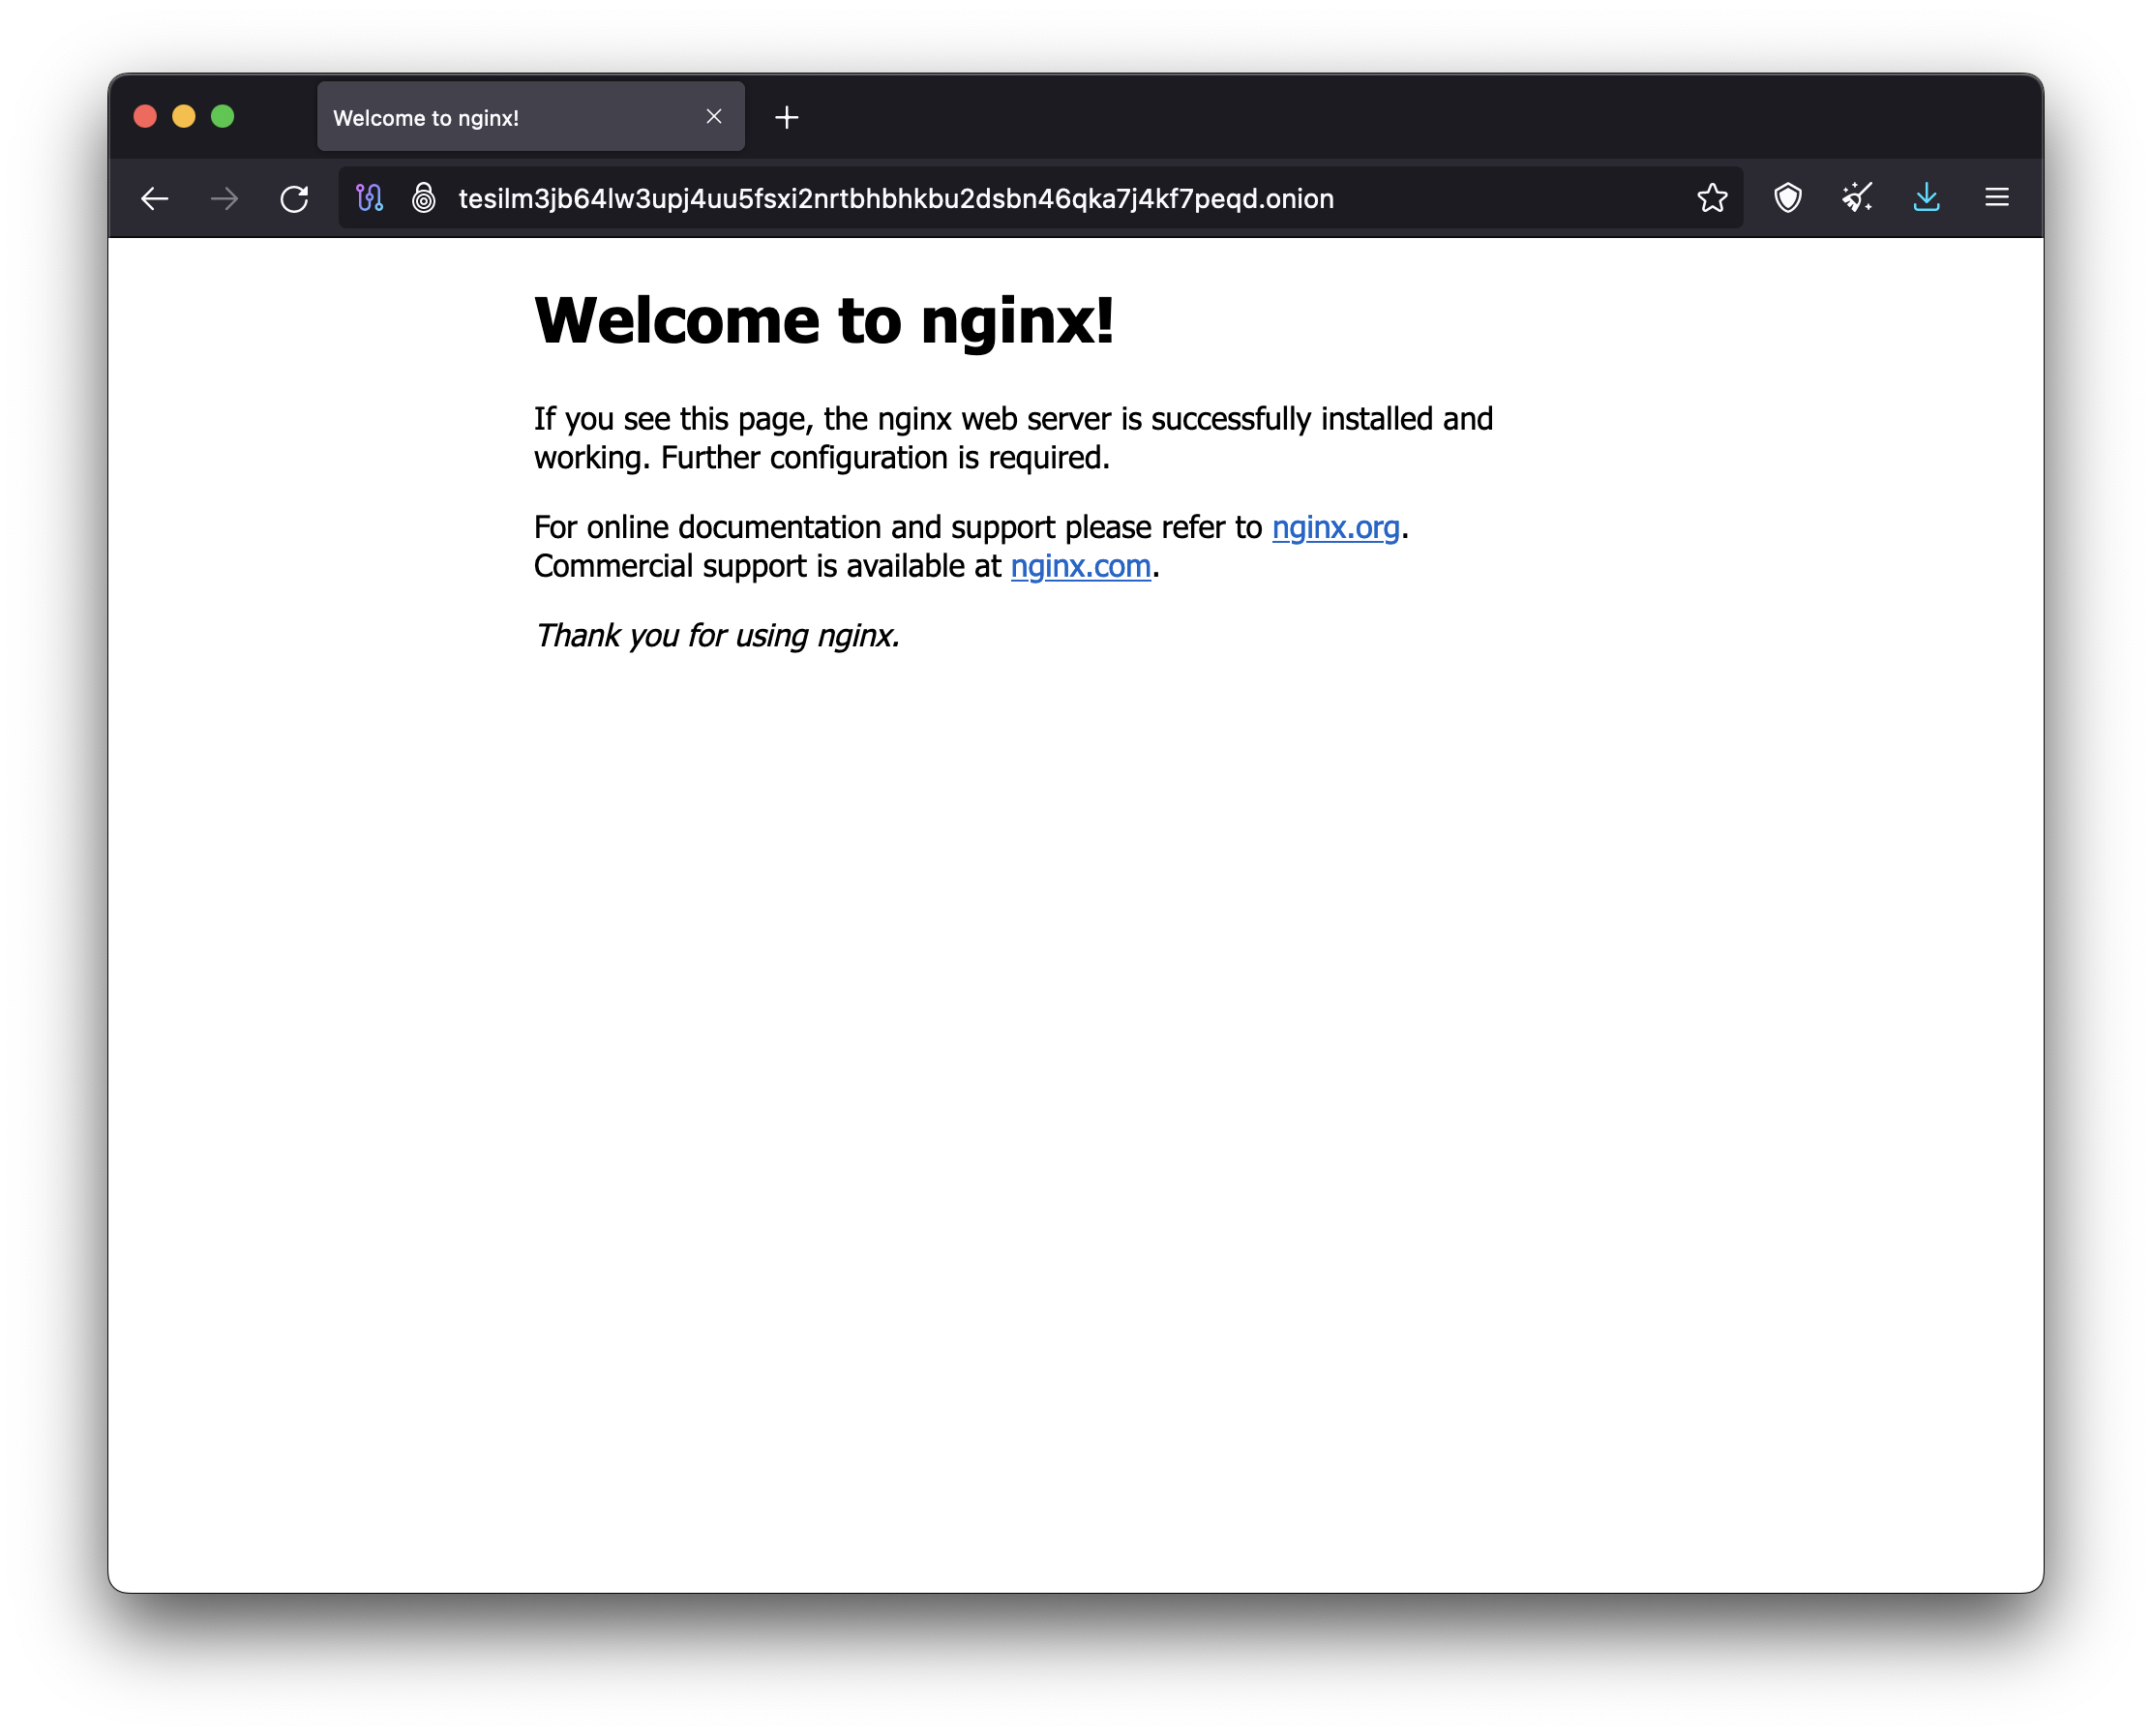
\includegraphics[width=\textwidth]{connectionCustomAddress}
    \caption{Connessione con il nuovo url}
}

\newpage

\subsection{Far conoscere il sito}
Un'altra caratteristica importante per ogni sito è la capacità di essere ricercato tramite un motore di ricerca, ci sono diversi motori che eseguono l'indexing. Tra questi c'è notevil\footnote{http://notevilmtxf25uw7tskqxj6njlpebyrmlrerfv5hc4tuq7c7hilbyiqd.onion} funziona come un classico motore di ricerca, a differenza di altri motori come Torch che invece esegue la ricerca più in base al contenuto che all'url\footnote{Un test di ricerca di 'proton mail' in entrambi mostra solo notEvil restituirci il sito corretto} \\
In NotEvil è possibile contattare gli amministratori del motore per richiedere l'aggiunta di un sito. Dalla pagina ufficiale è infatti presente il pulsante di contatto, dopo un breve controllo ci permette di inviare una richiesta anonima cosi che il sito possa essere analizzato ed aggiunto\\
Un'altro sistema per far conoscere il sito agli utenti finali è l'utilizzo di siti specializzati come OnionDir\footnote{https://oniondiricuc4x2y5qbucg4jyp2ael5rxy7aahy5f4fbars2jkkf7vad.onion.nz} che permette di aggiungere il proprio sito in maniera completamente anonima. \\
In questo caso basta cliccare sul tasto \lstinline{Add Link} nella toolbar in alto. \\
\importImage{
    \label{fig:OnionDir}
    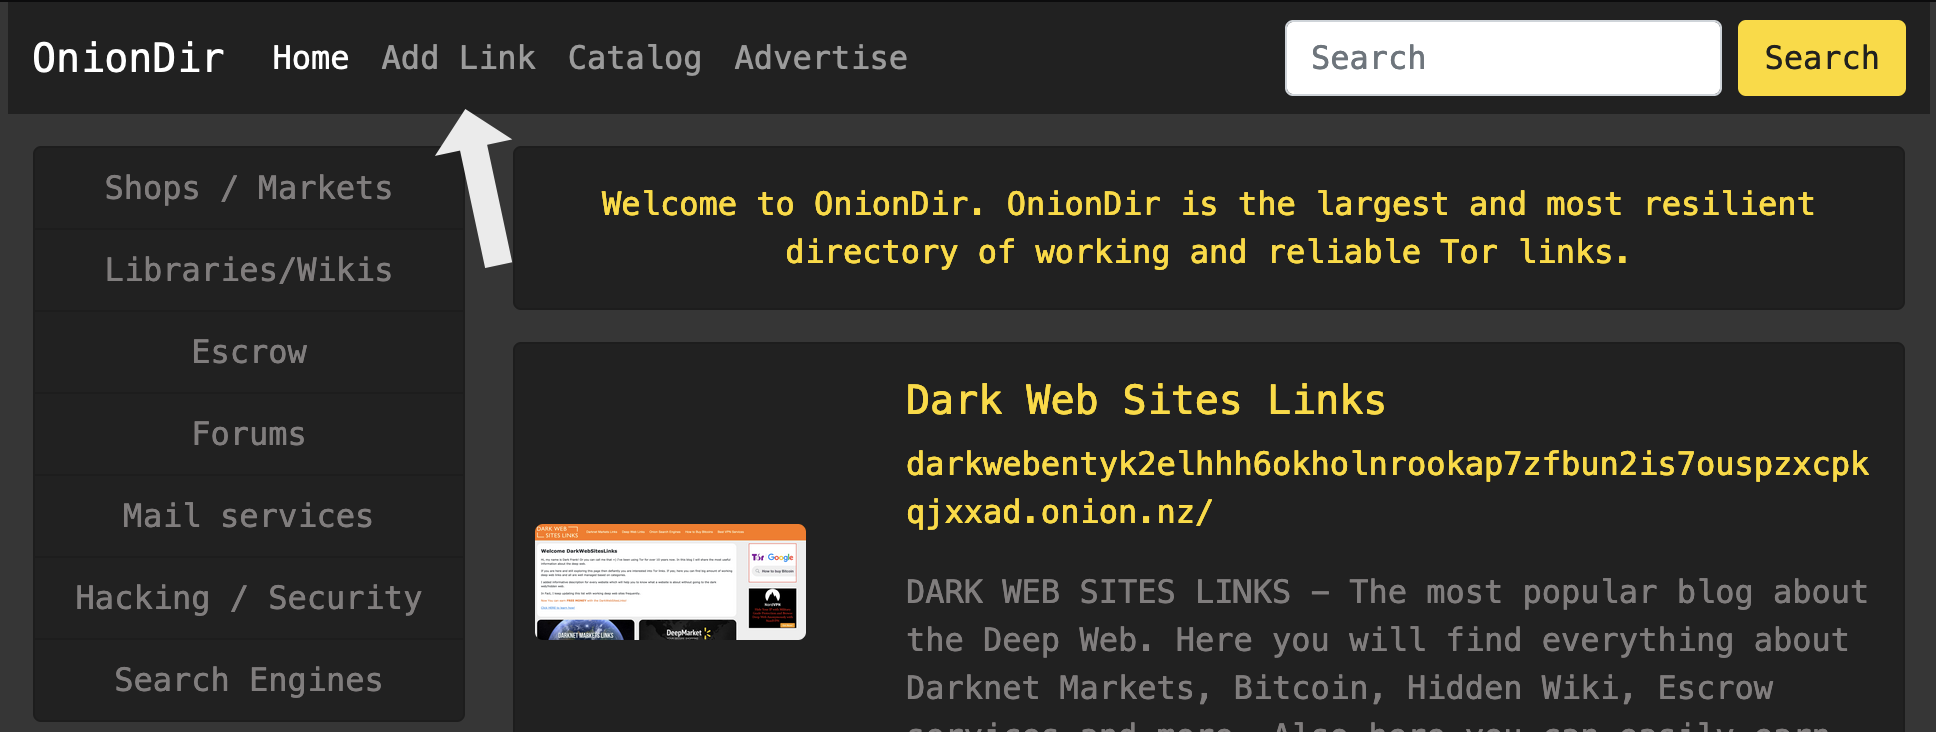
\includegraphics[width=\textwidth]{OnionDirMain}
    \caption{OnionDir, Pagina iniziale}
}
A questo punto possiamo inserire l'url e una piccola descrizione, come NotEvil il sito sarà scansionato per evitare truffe o contenuti proibiti, come indicato nelle poche righe di descrizione dei termini del servizio. \\
\importImage{
    \label{fig:OnionDirForm}
    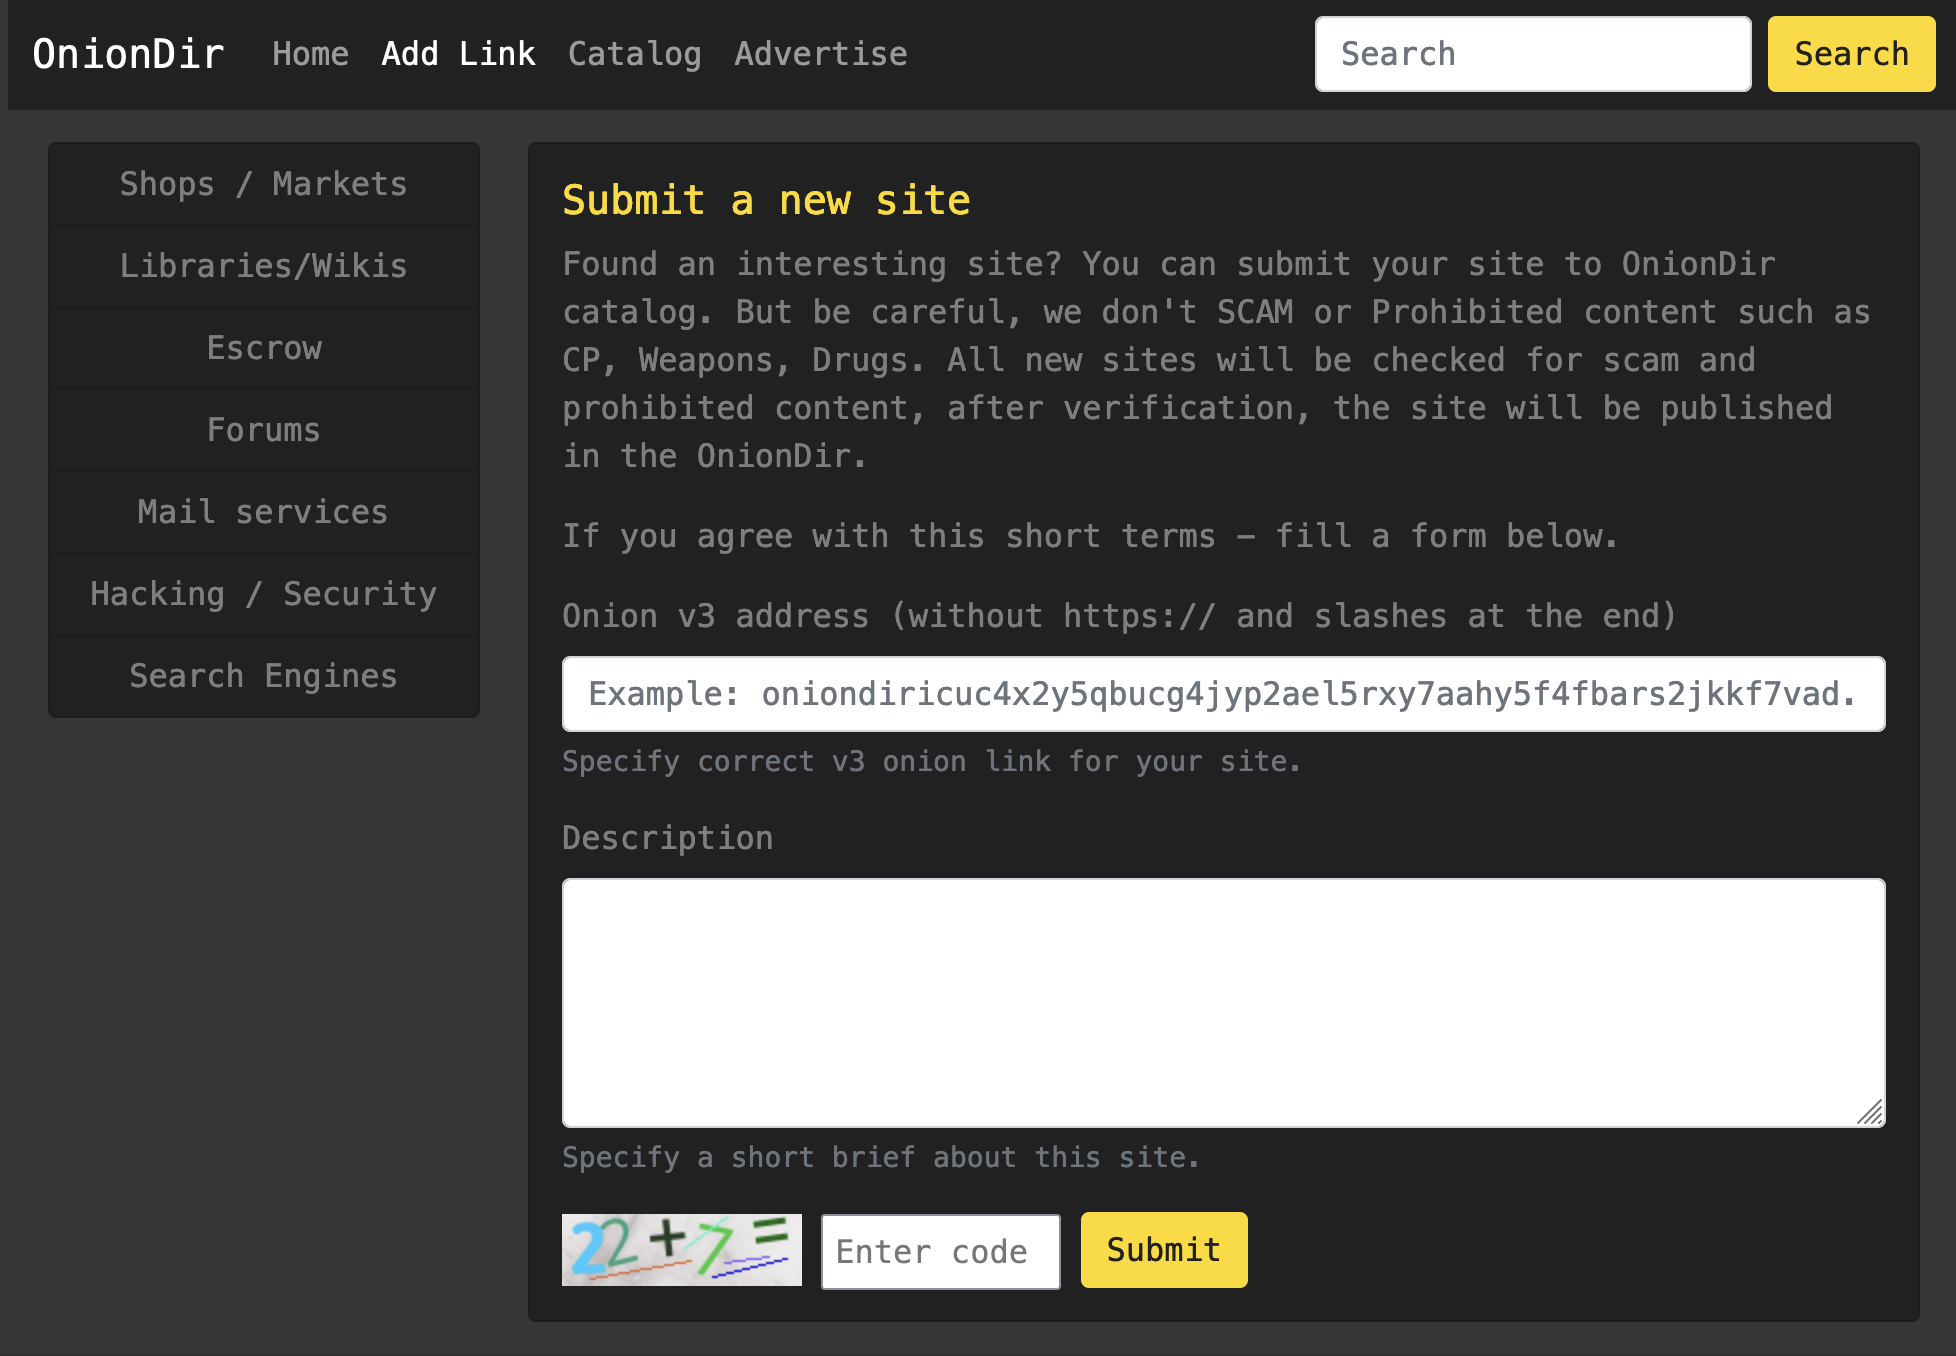
\includegraphics[width=\textwidth]{OnionDirForm}
    \caption{OnionDir, Form aggiunta sito}
}
    
    \chapter{Capitolo Esempio}
\label{chap:CapitoloEsempio}

Lorem ipsum dolor sit amet, consectetur adipisci elit, sed do eiusmod tempor incidunt ut labore et dolore magna aliqua. Ut enim ad minim veniam, quis nostrum exercitationem ullamco laboriosam, nisi ut aliquid ex ea commodi consequatur. Duis aute irure reprehenderit in voluptate velit esse cillum dolore eu fugiat nulla pariatur. Excepteur sint obcaecat cupiditat non proident, sunt in culpa qui officia deserunt mollit anim id est laborum.

In questo capitolo andremo a discutere ...
  
\section{Sezione Esempio}
\label{sec:real-time}
Quello in Figura \ref{fig:rocker}  (esempio di riferimento a figura) ...

% \begin{figure}[htpb!]
%   \centering
%   
\includegraphics[width=0.5\textwidth]{Rockerduck}
%   \caption{Esempio di figura}
%   \label{fig:rocker}
% \end{figure}

Esempio elenco puntato ...
\begin{itemize}
	\item item 1
	\item item 2
	\item item 3
\end{itemize}


\section{Section2}

\subsection{Subsection Esempio}
\label{sec:handshake}

\subsection{Subsection Esempio}
\label{sec:handshake}

\begin{lstlisting}[caption={Esempio di listing}, style=javaScriptCode]
	GET /chat HTTP/1.1
	Host: server.example.com
	Upgrade: websocket
	Connection: Upgrade
	Sec-WebSocket-Key: dGhlIHNhbXBsZSBub25jZQ==
	Origin: http://example.com
	Sec-WebSocket-Protocol: chat, superchat
	Sec-WebSocket-Version: 13
\end{lstlisting} 


\begin{table}[htbp]
	\begin{center}
		\begin{tabular}{|l|l|l|l|l|l|}
			\hline
			Versione & Chrome & Firefox & Internet Explorer & Opera & Safari \\
			\hline
			76 & 6 & 4.0 & No & 11.00(disabilitato) & 5.0.1\\
			\hline
			7 & No & 6.0 & No & No & No \\
			\hline
			10 & 14 & 7.0 & HTML5 Labs & ? & ?\\
			\hline
			RFC 6455 & 16 & 11.0 & 10 & 12.10 & 6.0\\
			\hline
		\end{tabular}
	\end{center}
	\caption{Esempio di Tabella}
	\label{tab:browser}
\end{table}

\begin{table}[htbp]
	\begin{center}
		\begin{tabular}{|l|l|l|l|l|l|}
			\hline
			Versione & Android & Firefox Mob. & IE Mob. & Opera Mob. & Safari Mob.\\
			\hline
			76 & ? & ? & ? & ? & ?\\
			\hline
			7 & ? & ? & ? & ? & ? \\
			\hline
			10 & ? & 7.0 & ? & ? & ?\\
			\hline
			RFC 6455 & 16(Chrome) & 11.0 & ? & 12.10 & 6.0\\
			\hline
		\end{tabular}
	\end{center}
	\caption{Esempio di Tabella}
	\label{tab:mobile}
\end{table}
Nelle Tabelle \ref{tab:browser} e \ref{tab:mobile} è possibile vedere, rispettivamente per desktop e per mobile, il supporto dei vari browser per le diverse specifiche delle WebSocket.
Il codice completo dell'esempio è disponibile sul mio GitHub\footnote{\url{https://github.com/Glydric/TesiTriennale}} (Esempio di link).

\section{Qui}


Ciao Ciao

\newpage
Ciao Ciao


Ciao Ciao

\makeatother

% \appendix
%\input{schema_elettrico}
%\input{Appendix1}
%\input{Appendix2}

\printbibliography

\printindex

\chapter*{Ringraziamenti}

In primo luogo vorrei ringraziare il Professore Fausto Marcantoni, non solo per avermi dato la possibilità di lavorare a questa tesi, ma anche per avermi fatto appassionare alla materia e ai suoi insegnamenti. \\
Ringrazio i miei genitori, per avermi sempre sostenuto ed insieme ai miei nonni per avermi permesso di studiare e di arrivare fino a questo punto. \\


\end{document}